%%%%%%%%%%%%%%%%%%%%%%%%%%%%%%%%%%%%%%%%%

%\title{Title page with logo}
%----------------------------------------------------------------------------------------
%	PACKAGES AND OTHER DOCUMENT CONFIGURATIONS
%----------------------------------------------------------------------------------------

\documentclass[12pt]{article}
\usepackage[portuguese]{babel}
\usepackage[utf8x]{inputenc}
\usepackage{amsmath}
\usepackage{amssymb}
\usepackage{graphicx}
\usepackage{natbib}
\usepackage{cite} 
\usepackage{float}
\usepackage{calrsfs}
\usepackage[a4paper,left=2.5cm,right=2.5cm,top=2.5cm, bottom=2.5cm]{geometry}
\usepackage{verbatim}
\usepackage{bigints}
\usepackage{booktabs}
\usepackage[table]{xcolor}
\usepackage{siunitx}

\begin{document}

\begin{titlepage}

\newcommand{\HRule}{\rule{\linewidth}{0.5mm}} % Defines a new command for the horizontal lines, change thickness here

\center % Center everything on the page
 
%----------------------------------------------------------------------------------------
%	HEADING SECTIONS
%----------------------------------------------------------------------------------------

\textsc{\LARGE Universidade Federal de Alagoas}\\[1.5cm] % Name of your university/college
\textsc{\Large Instituto de Computação (IC)}\\[0.5cm] % Major heading such as course name
\textsc{\large Laboratório de Computação Científica e Análise Numérica (LaCCAN)}\\[3.5cm] % Minor heading such as course title

%----------------------------------------------------------------------------------------
%	TITLE SECTION
%----------------------------------------------------------------------------------------

\HRule \\[0.4cm]
{ \LARGE \bfseries Estimadores dos parâmetros para a Distribuição $G_I^0$}\\[0.4cm] 
\HRule \\[2.5cm]
 
%----------------------------------------------------------------------------------------
%	AUTHOR SECTION
%----------------------------------------------------------------------------------------

\begin{minipage}{0.4\textwidth}
\begin{flushleft} \large
\emph{Autor:}\\
Marcos G. S. do Nascimento % Your name
\end{flushleft}
\end{minipage}
~
\begin{minipage}{0.4\textwidth}
\begin{flushright} \large
\emph{Orientador:} \\
Alejandro C. Frery  % Supervisor's Name
\end{flushright}
\end{minipage}\\[8cm]

% If you don't want a supervisor, uncomment the two lines below and remove the section above
%\Large \emph{Author:}\\
%John \textsc{Smith}\\[3cm] % Your name

%----------------------------------------------------------------------------------------
%	DATE SECTION
%----------------------------------------------------------------------------------------

{\large 24/10/2018}\\[2cm] % Date, change the \today to a set date if you want to be precise

%----------------------------------------------------------------------------------------
%	LOGO SECTION
%----------------------------------------------------------------------------------------

% \includegraphics{logo.png}\\[1cm] % Include a department/university logo - this will require the graphicx package
 
%----------------------------------------------------------------------------------------

\vfill % Fill the rest of the page with whitespace

\end{titlepage}


\section{Introdução}
%%% ACF Evite usar "\\" e qualquer outra formatação fixa

Conforme \citet{FreryMinute2004}, o sensoriamento remoto por microondas pode ser usado para obter informações sobre cenas inacessíveis e/ou não observáveis. A superfície de Vênus, remota e invisível devido à constante cobertura de nuvens, foi mapeada usando sensores de radar. Sensores semelhantes, ou seja, radares de abertura sintética (SARs) são usados para monitorar regiões terrestres inacessíveis, como a Amazônia, os polos e assim por diante. Imagens de ultra-som B são empregadas para diagnosticar sem invadir o corpo. Imagens de sonar são usadas para mapear o fundo do mar, lagos e rios profundos ou escuros, e a iluminação a laser pode ser usada para rastrear perfis de entidades microscópicas.

Essas imagens são formadas por sensores ativos (já que carregam sua própria fonte de iluminação) que enviam e recuperam sinais cuja fase é registrada, ou seja, são  obtidas com radiação coerente. As imagens são formadas detectando o eco do alvo (backscatter) e, nesse processo, um ruído é introduzido devido a fenômenos de interferência. A esse ruído, damos o nome de $speckle$. As propriedades do ruído ($speckle$) são bem descritas pelo modelo multiplicativo, uma estrutura estatística a partir da qual derivam várias distribuições importantes. Entre essas distribuições, uma é considerada o Modelo Universal para dados ruidosos, a saber, a lei $G^{0}$. Esse relatório aborda dados em intensidade, então a distribuição $G_I^0$ será utilizada na estimação dos parâmetros.

\section{O Modelo Universal (Lei $G^{0}$)}

A modelagem estatística dos dados é essencial para interpretar imagens SAR. O artigo de pesquisa de \citet{Gao2010StatisticalMO} discute em detalhes vários modelos estatísticos para esse tipo de dado.
%%% ACF Por que o sobrenome GAO aparece em maiúsculas?

%%% ACF Use modo matemático
Segundo \citet{Mejail2002}, dentre os modelos estatísticos disponíveis, o modelo multiplicativo baseia-se no pressuposto de que o campo aleatório observado (retorno) $Z$ é o resultado do produto de dois campos aleatórios independentes e não observados: $X$ e $Y$. O campo aleatório $X$ modela o retroespalhamento (\textit{backscatter})  do terreno e, portanto, depende apenas do tipo de área a que cada pixel pertence. O campo aleatório $Y$ leva em consideração que as imagens SAR são o resultado de um sistema de geração de imagens coerente que produz o conhecido fenômeno chamado ruído $speckle$, e que elas são geradas pela média de $n$ imagens (teoricamente independentes) - $looks$ - para reduzir o efeito do \textit{speckle}.

Conforme proposto e avaliado em \citet{Clutter1997}, as distribuições $G^0$ podem ser utilizadas com sucesso para descrever os dados contaminados pelo ruído (\textit{speckle}). Dessa forma, os dados ruidosos foram descritos no modelo multiplicativo usando a família $G$ de distribuições que é capaz de descrever áreas extremamente  melhor que a distribuição $K$. Foi demonstrado que essa classe de distribuições é capaz de caracterizar um grande número de alvos em imagens de SAR monopolarizadas, merecendo a denominação de “Modelo Universal”. 

\subsection{Introdução ao Modelo $G_I^0$}

Segundo \citet{FreryStochasticDistances2015}, o modelo $G_I^0$ é indexado por três parâmetros: o número de $Looks$ ($L$) que pode ser estimado em toda a imagem, um parâmetro de escala ($\gamma$) e o parâmetro de rugosidade ou textura ($\alpha$). Este último está intimamente relacionado ao número de $backscatters$ elementares em cada pixel, uma das razões para receber atenção na literatura. Embora haja esforços em fornecer estimativas aprimoradas e robustas para tal quantidade, sua estimativa confiável ainda apresenta problemas numéricos na prática. Vale ressaltar ainda que o número de $Looks$ consiste em um parâmetro que pode ser controlado no processo de geração de imagens e, portanto, será considerado conhecido. Este parâmetro está relacionado à relação sinal-ruído e à precisão espacial da imagem.

Como discutido anteriormente sobre o Modelo Multiplicativo, o retorno em imagens SAR monopolarizadas pode ser modelado como o produto de duas variáveis aleatórias independentes, uma correspondendo ao $backscatter$ $X$ e a outra ao $speckle$ $Y$. Desta maneira, $Z = XY$ representa o retorno em cada pixel sob o modelo multiplicativo. 

Para dados monopolarizados e no caso da distribuição $G_I^0$, o $speckle$ é modelado como uma variável aleatória $Gama$ ($\Gamma$), com média unitária e parâmetro de forma $L \geq 1$, que corresponde ao número de $Looks$, ou seja, o $speckle$ é modelado seguindo a distribuição dada por $\Gamma(L,1)$. O \textit{backscatter}, por sua vez, é considerado obedecendo a uma recíproca da lei $Gama$, isto é, $\Gamma^{-1}(\alpha,\gamma)$. 

Temos que, se $Z \sim G_I^0(\alpha, \gamma, L)$, então sua função de densidade de probabilidade é dada por
%%% ACF Não deixe espaço antes de elementos que fazem parte do parágrafo. Repare no uso de \text
\begin{equation}
    f_Z(z; \alpha, \gamma, \textit{L})= \frac{L^L\Gamma(L-\alpha)z^{L-1}}{\gamma^\alpha\Gamma(-\alpha)\Gamma(L)(\gamma + zL)^{L-\alpha}} \label{eq:fdpGI0}
\end{equation}
onde $-\alpha, \gamma, z > 0$ e $L \geq 1$. $\Gamma$, neste caso, representa a função $gama$. Os parâmetros $\alpha$ e $\gamma$ nesta função de densidade são os parâmetros desconhecidos.

Por sua vez, os momentos de ordem $r$ ($r$-order moments) são dados por
\begin{equation}
    E(Z^r) = \left (\frac{\gamma}{L}\right )^{r}\frac{\Gamma(-\alpha-r)\Gamma(L+r)}{\Gamma(-\alpha)\Gamma(L)} \label{eq:moments}
\end{equation}
fornecidos dessa forma se $\alpha < -r$, e são infinitos, caso contrário.

No processo de estimação, podemos fazer simplificações para reduzir a complexidade dos cálculos e tornar os resultados comparáveis. Para isso, por exemplo, podemos escolher o parâmetro de escala ($\gamma$) de modo que se tenha $E(Z) = 1$, que é dado por $\gamma* = -\alpha - 1$. 

Uma característica crucial da distribuição caracterizada por \eqref{eq:fdpGI0} é que seus parâmetros são interpretáveis: $\gamma$ é um parâmetro de escala e o número de $Looks$ é conhecido antecipadamente ou é estimado para a imagem inteira usando alvos estendidos (amostras muito grandes). Uma das características mais importantes da distribuição $G_I^0$ é a interpretação de seu parâmetro $\alpha$ que está relacionado com a rugosidade do alvo. Valores próximos de $0$ (tipicamente acima de $-3$) sugerem alvos extremamente texturizados, como zonas urbanas. Em situações intermediárias, à medida que o valor diminui, isso indica regiões com textura moderada (geralmente $\alpha \in  [−6, −3]$), tipicamente áreas irregulares, como zonas florestais. Alvos sem textura, geralmente produzem $\alpha \in (−\infty, −6)$ como é o caso de regiões lisas, por exemplo, pastagem, culturas e campos queimados. Esta é a razão pela qual a precisão na estimativa de $\alpha$ é tão importante.

A figura a seguir apresenta as curvas de densidade da distribuição $G_I^0$ para determinados parâmetros.
% GI0 Densities
\begin{figure}[H]
     \centering
     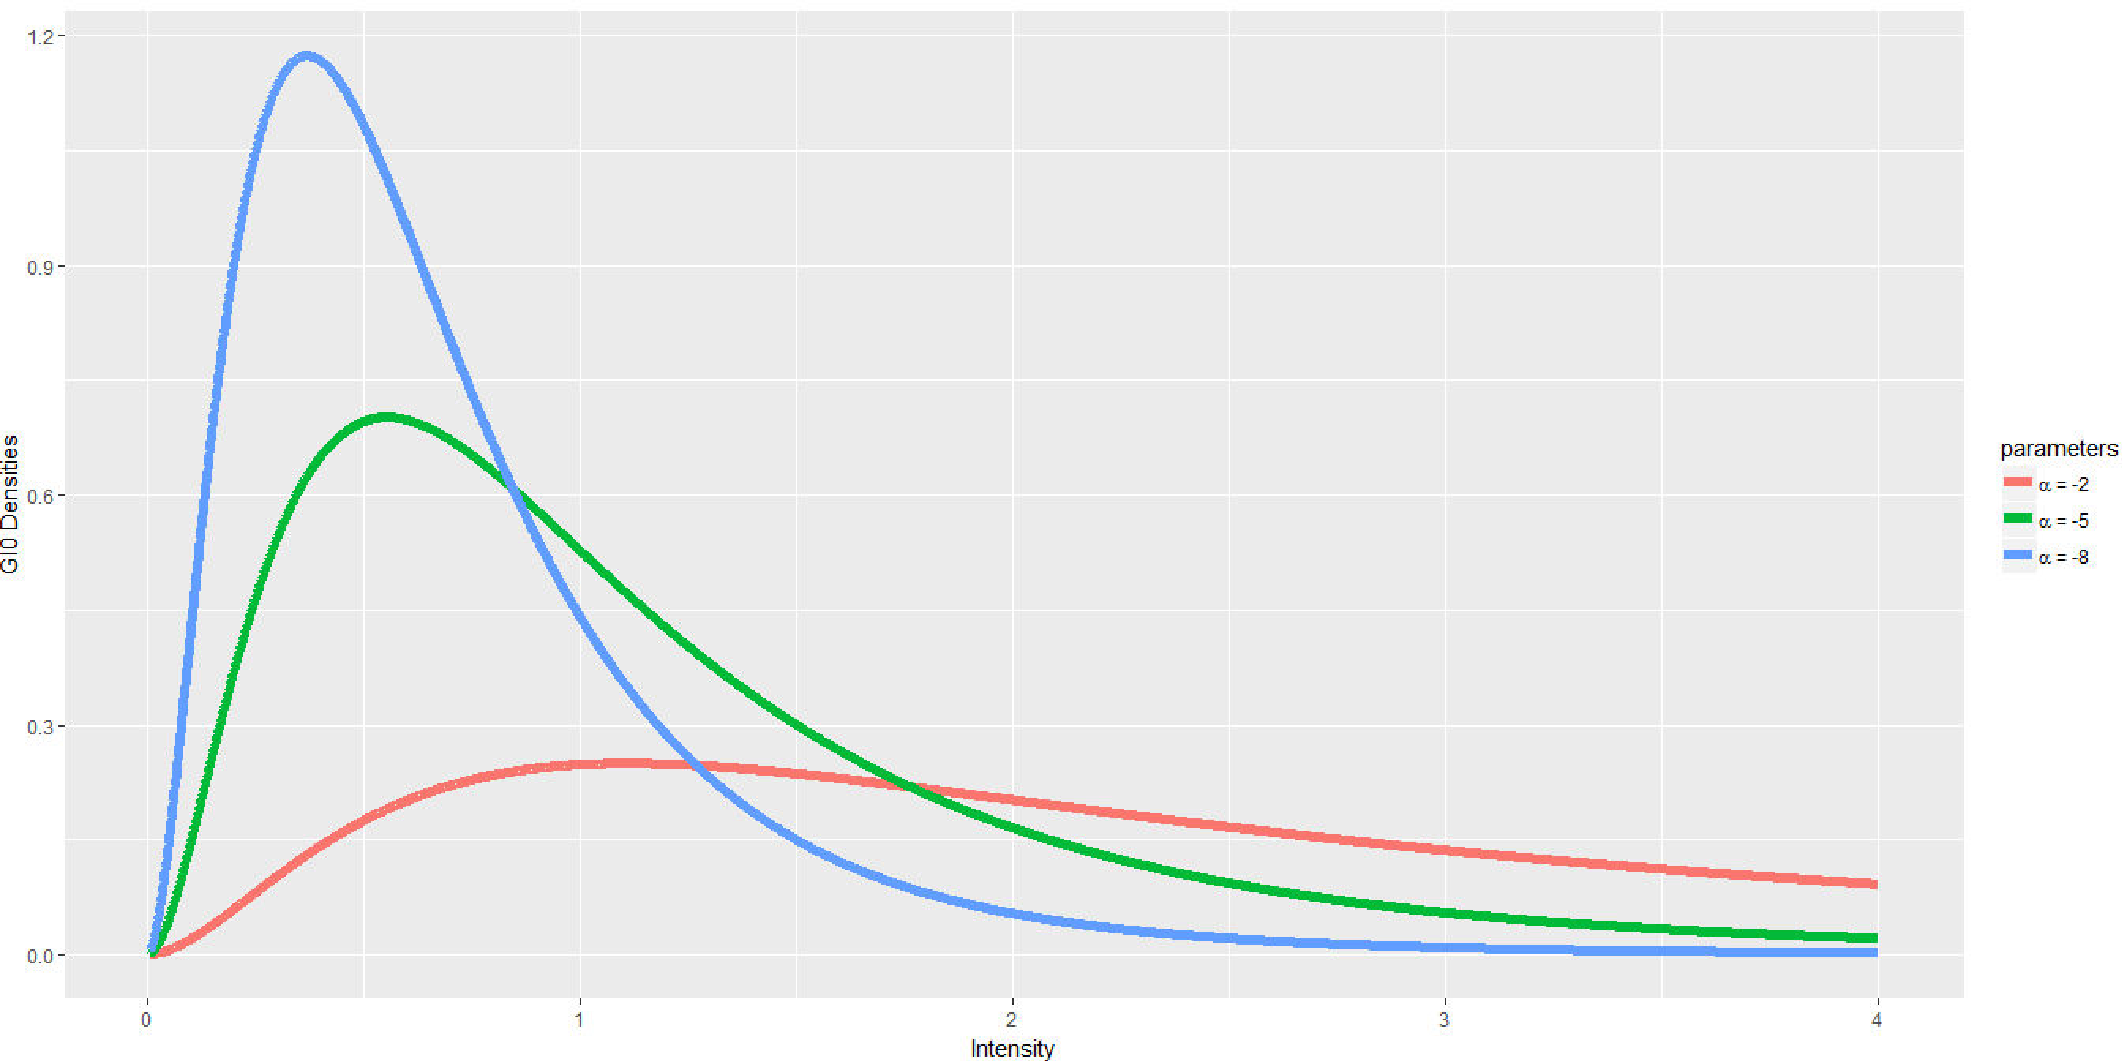
\includegraphics[scale=0.5]{plots/GI0Densities.pdf}
     \caption{Densidades da distribuição $G_I^0(\alpha, 5, 3)$, com $\alpha \in \left \{  -8, -5, -2 \right \}$}
     \label{graf_1}
\end{figure}

Vale reforçar que Sistemas que empregam iluminação coerente são usados para explorar regiões inacessíveis e/ou inobserváveis (a superfície de Vênus, o interior do corpo humano, o fundo do mar, áreas sob nebulosidade, etc.). É, portanto, de suma importância poder fazer inferências confiáveis sobre o tipo de alvo em análise, uma vez que informações visuais raramente estão disponíveis.


\subsection{Estimação por Máxima Verossimilhança (MV)}

As técnicas usuais de inferência incluem métodos baseados no princípio de analogia, sendo os estimadores estatísticos de ordem e momento os mais populares desta classe, e no princípio de Máxima Verossimilhança (MV). Estimadores de momentos são favorecidos em aplicações, já que são fáceis de derivar e são, geralmente, computacionalmente atraentes. Os estimadores MV são amplamente utilizados, uma vez que possuem propriedades ótimas bem conhecidas, como consistência, eficiência e normalidade assintótica, entre outras. Esses estimadores foram utilizados para a análise de imagens de SAR sob o modelo $K$ no trabalho de \citet{KMaxVer_Joughin}.

Dado uma amostra $Z = (Z_1, Z_2, \dots, Z_N)$ e assumindo que essas observações são resultados de variáveis aleatórias independentes e identicamente distribuídas que seguem a distribuição $D(\theta)$, com $\theta \in \Theta$, um estimador MV para $\theta$ é dado por
%%% ACF Use \arg\max
\begin{equation}
    \widehat{\theta} = \arg\max L(\theta; z) \quad \text{para} \quad \theta \in \Theta, \label{eq:mv}
\end{equation}
em que $L$ é a função de verossimilhança da amostra $Z$ sob o parâmetro $\theta$. Podemos utilizar as propriedades logarítmicas para simplificar os cálculos, aplicando o logaritmo natural, visto que o ponto que produz o máximo da função não varia, independentemente de aplicar o logaritmo. Além disso, sob várias condições é equivalente e muitas vezes mais fácil trabalhar com a função log-verossimilhança reduzida $l(\theta; Z)$, onde todos os termos que não dependem de $\theta$ são ignorados.

Embora a maximização direta de \eqref{eq:mv} seja possível (seja analiticamente ou usando ferramentas numéricas) e desejável, muitas vezes encontramos estimadores de MV resolvendo o sistema de equações (geralmente não-lineares) dado por
\begin{equation}
    \nabla l(\widehat{\theta}) = 0 \label{eq:gradient} 
\end{equation}
onde, neste caso, $\nabla$ denota o gradiente. Segundo \citet{FreryMinute2004}, a escolha entre resolver \eqref{eq:mv} ou \eqref{eq:gradient} depende muito de questões computacionais: disponibilidade de algoritmos confiáveis, esforço computacional necessário para implementar e/ou obter a solução e assim por diante. Essas equações, em geral, não têm solução explícita.

Para a construção dos estimadores de Máxima Verossimilhança para o modelo $G_I^0$, considere $Z = (Z_1, Z_2, \dots, Z_N)$ uma amostra aleatória de $N$ variáveis, independentes e igualmente distribuídas, que seguem essa distribuição. Os parâmetros $\alpha$ e $\gamma$ são desconhecidos, enquanto que o parâmetro $Looks$ é conhecido. Nesse caso, a função de verossimilhança é $L((\alpha, \gamma); Z) = \prod_{i=1}^{N} f_Z(Z_i)$, onde $f_Z$ é a função densidade de probabilidade definida anteriormente em \eqref{eq:fdpGI0}. 

Assim, a função de log-verossimilhança ($\log L$) é escrita como
\begin{equation}
    \log L((\alpha, \gamma); Z) = N\log \frac{L^{L}\Gamma(L-\alpha)}{\gamma^{\alpha}\Gamma(-\alpha)\Gamma(L)} +  (L-1)\sum_{i=1}^{N}\log Z_i - (L-\alpha)\sum_{i=1}^{N}\log (\gamma + Z_iL) \label{eq:logVer}
\end{equation}

A partir da função acima, podemos escrever a função de log-verossimilhança reduzida ($l$), excluindo os termos que não dependem de $\alpha$ e $\gamma$
\begin{equation}
    l((\alpha, \gamma); Z) = N\log\Gamma(L-\alpha) - N\alpha \log\gamma - N\log\Gamma(-\alpha) - (L-\alpha)\sum_{i=1}^{N}\log(\gamma +Z_iL) \label{eq:logVerRed}
\end{equation}

O sistema de equações representado em \eqref{eq:gradient} é, em nosso caso, dado por
\begin{equation}
  \frac{\partial l}{\partial \widehat{\alpha}} = N[\Psi(-\widehat{\alpha}) - \Psi(L-\widehat{\alpha})] + \sum_{i=1}^{N}\log\frac{\widehat{\gamma} + Z_iL}{\widehat{\gamma}} = 0
\end{equation}
\begin{equation}
   \frac{\partial l}{\partial \widehat{\gamma}} = -N\frac{\widehat{\alpha}}{\widehat{\gamma}} - (L - \widehat{\alpha})\sum_{i=1}^{N}(\widehat{\gamma} + Z_iL)^{-1} = 0
\end{equation}
em que $\Psi(\tau) = \frac{\textit{d}log\Gamma(\tau)}{\textit{d}\tau}$ é a função $Digama$. Resolvendo esse sistema de equações obtemos os estimadores para os parâmetros $\alpha$ e $\gamma$ da distribuição $G_I^0$, denotados por $\widehat{\alpha}$ e $\widehat{\gamma}$. Em geral, nenhuma solução explícita para este sistema está disponível e, portanto, rotinas numéricas têm que ser usadas.

Assumindo a simplificação feita para o parâmetro de escala ($\gamma* = -\alpha - 1$), temos que o estimador de Máxima Verossimilhança para o parâmetro $\alpha$, chamado $\widehat{\alpha}$, é dado pela solução da seguinte equação não linear:
\begin{eqnarray}
    \Psi(-\widehat{\alpha}) - \Psi(L-\widehat{\alpha}) - \log(-\widehat{\alpha}-1) - \frac{\widehat{\alpha}}{\widehat{\alpha}+1} + \nonumber \\ \frac{1}{N}\sum_{i=1}^{N}\log(-\widehat{\alpha} - 1 + LZ_i) - \left ( \frac{\widehat{\alpha}-L}{N} \right )\sum_{i=1}^{N}(-\widehat{\alpha} - 1 + LZ_i)^{-1} & = & 0
\end{eqnarray}

\subsection{Estimação pelo Método dos Momentos (MM)}

Uma outra forma de encontrar estimadores de parâmetros populacionais, como a média e a variância por exemplo, é através do método dos momentos. Este método é baseado na comparação dos momentos teóricos com os momentos amostrais das variáveis aleatórias envolvidas, a partir de uma amostra de $N$ observações.

Seja $Z$ uma variável aleatória contínua com função densidade de probabilidade $f_Z(z)$, os momentos teóricos são dados por $m_j = \int x^jf_Z(z)dz$. Os momentos amostrais, por sua vez, são definidos como $\widehat{m_j} = N^{-1}\sum_{i=1}^{N}z_i^j$. O índice $\textit{j}$ representa a ordem do momento. Após calcular os momentos teóricos e amostrais, o processo de inferência é simples e consiste em comparar os momentos amostrais, $\widehat{m_j}$, com os correspondentes momentos teóricos, $m_j$, até se ter tantas equações quantos forem os parâmetros a serem estimados. De posse do sistema de equações, basta resolver e calcular os estimadores para os parâmetros.

Para estimar os parâmetros $\alpha$ e $\gamma$ da distribuição $G_I^0(\alpha, \gamma, L)$, é necessário estimar dois momentos. Neste relatório, serão utilizados momentos de ordem $\frac{1}{2}$ e $1$, ou seja, $m_{1/2}$ e $m_1$ respectivamente. Esses momentos, de acordo com a equação \eqref{eq:moments}, são dados por
\begin{equation}
    m_{1/2} = \left ( \frac{\gamma}{L}\right )^{1/2} \frac{\Gamma(-\alpha-1/2)\Gamma(L+1/2)}{\Gamma(-\alpha)\Gamma(L)} \quad \text{para} \quad \alpha < -1/2 \label{eq:m12}
\end{equation}
\begin{equation}
    m_{1} = \left ( \frac{\gamma}{L}\right ) \frac{\Gamma(-\alpha-1)\Gamma(L+1)}{\Gamma(-\alpha)\Gamma(L)} \quad \text{para} \quad \alpha < -1 \label{eq:m1}
\end{equation}

Podemos utilizar o momento $\widehat{m}_{1/2}^2$ para auxiliar nos cálculos e utilizar as equações acima \eqref{eq:m12} e \eqref{eq:m1} para determinar o estimador $\widehat{\alpha}$ que pode ser dado como solução da seguinte equação
\begin{equation}
    g(\widehat{\alpha}) - \zeta = 0
\end{equation}
onde 
\begin{equation}
    g(\widehat{\alpha}) = \frac{\Gamma^2(-\widehat{\alpha} - 1/2)}{\Gamma(-\widehat{\alpha})\Gamma(-\widehat{\alpha} - 1)}
\end{equation}
e
\begin{equation}
    \zeta = \frac{\widehat{m}_{1/2}^2\Gamma(L)\Gamma(L+1)}{\widehat{m}_{1}\Gamma^2(L+1/2)}
\end{equation}
Dessa forma, encontrando o valor de $\widehat{\alpha}$ e o substituindo na equação \eqref{eq:m12} ou na equação \eqref{eq:m1}, obtemos o estimador $\widehat{\gamma}$.

Como já mencionado, podemos simplificar o processo de estimação do parâmetro $\gamma$, obtendo-o este de tal forma que o valor esperado $E(Z^r)$ tenha valor unitário e, assim, definimos ele em função do parâmetro $\alpha$. Dessa forma, podemos encontrar $\gamma*$ a partir de \eqref{eq:moments} como a seguir
\begin{equation}
    E(Z^r) = 1 \Rightarrow \left (\frac{\gamma*}{L}\right ) \frac{\Gamma(-\alpha-1)\Gamma(L+1)}{\Gamma(-\alpha)\Gamma(L)} = 1 \Rightarrow \gamma* = L\left ( \frac{\Gamma(-\alpha)\Gamma(L)}{\Gamma(-\alpha-1)\Gamma(L+1)} \right ) 
\end{equation}
onde, fazendo $\Gamma(n) = (n-1)!$, temos
\begin{equation}
    \gamma* = -\alpha - 1
\end{equation}
Estimadores de momentos fracionários foram utilizadas amplamente em \citet{Clutter1997}. Dessa forma, assumindo a simplificação acima e utilizando $r=\frac{1}{2}$ na equação do $r$-ésimo momento da $G_I^0$ dada em \eqref{eq:moments} é preciso resolver a equação a seguir para se obter o estimador $\widehat{\alpha}$
\begin{equation}
    \frac{1}{N}\sum_{i=1}^{N}\sqrt{z_i}-\sqrt{\frac{-\widehat{\alpha} - 1}{L}}\frac{\Gamma(-\widehat{\alpha} - \frac{1}{2})}{\Gamma(-\widehat{\alpha})}\frac{\Gamma(L+\frac{1}{2})}{\Gamma(L)} = 0 \label{fractional_moments}
\end{equation}

\section{Estimação pelo Método de Log-Cumulantes (MLC)}

Sabe-se que a estimação de parâmetros de funções de densidade de probabilidade é um dos principais passos na área de processamento de imagens e sinais estatísticos. Nesse contexto, o método de log-cumulantes (MLC) consiste em um método de estimação de parâmetros proposto por \citet{nicolas2002} e tem sido utilizado com resultados satisfatórios em processamentos de imagens SAR.

O Método de Log-cumulantes pode ser visto como uma alternativa às abordagens clássicas de máxima verossimilhança (MV) e método dos momentos (MM). Estudos feitos no trabalho de \citet{krylov2013} derivaram uma condição geral suficiente para uma consistência forte das estimativas de MLC, que representa uma importante propriedade assintótica de qualquer estimador estatístico. Este resultado permite a demonstração da forte consistência das estimativas de MLC para uma seleção de famílias de distribuição amplamente utilizadas originárias de processamento de imagem de radar de abertura sintética, contudo não é restrito somente a esse campo. 

Nesse sentido, estimadores baseados em log-cumulantes têm ganhado espaço na literatura devido às suas boas propriedades e bom desempenho. No contexto de processamento de imagens SAR, este método é especialmente utilizado quando se tem pequenas amostras que se trata de um problema crítico em várias aplicações. Ainda no trabalho de \citet{krylov2013}, foram destacados que os resultados obtidos sugerem que o MLC é uma alternativa viável e computacionalmente rápida que é especialmente útil quando a abordagem direta do estimador de Máxima Verossimilhança se mostra inviável. 

Pesquisadores têm utilizado os parâmetros estimados pelo método de log-cumulantes como entradas, por exemplo, para métodos de classificação de imagens SAR e detecção de mudanças em imagens SAR multitemporais. A seguir é apresentado o MLC conforme proposto e analisado no trabalho de \citet{nicolas2002}.

Seja $Z$ uma variável aleatória contínua com função densidade de probabilidade $f_Z(z, \theta)$ definida em $\mathbb{R}^{+}$. O Método de log-cumulantes, baseado na transformada de Mellin de $f_Z(z, \theta)$, é definido como:
\begin{equation}
    \phi_{Z}(s) = \int_{0}^{\infty} u^{s-1} f_{Z}(u, \theta)\mathrm{d}u = E(Z^{s-1}) \label{eq:logcum}
\end{equation}
com s sendo um número complexo com norma unitária (\citet{nicolas2002})

Existem dois conceitos importantes para a construção de estimadores utilizando o método de log-cumulantes que são os log-momentos e log-cumulantes de ordem $v$. É possível obter expressões analíticas para os log-momentos e log-cumulantes de ordem $v$ por simples derivações de $\phi_{Z}(s)$, avaliadas em $s = 1$. O log-momento de ordem $v$ pode ser definido como:
\begin{equation}
    \tilde{m}_{v} = \frac{\mathrm{d}^{v}\phi_{Z}(s)}{\mathrm{d}s^{v}}\Bigr|_{\substack{s=1}} \quad , \quad  v \in \mathbb{N}
    \label{eq:logmomV}
\end{equation}

Tomando como base o logaritmo natural($ln$) de $\phi_{Z}(s)$, pode-se obter o log-cumulante de ordem $v$ de forma bem similar e análoga à equação anterior. Temos que:
\begin{equation}
    \tilde{k}_{v} = \frac{\mathrm{d}^{v}\psi_Z(s)}{\mathrm{d}s^{v}}\Bigr|_{\substack{s=1}} \quad , \quad  v \in \mathbb{N}
    \label{eq:logcumV}
\end{equation}
com $\psi_Z(s) = \log(\phi_{Z}(s))$.

O funcionamento e estratégia do método de log-cumulantes para estimar o vetor de parâmetros desejado $\theta$ se baseia na relação entre os log-momentos e log-cumulantes que é dada pela seguinte equação:
\begin{equation}
    \tilde{k}_{v} = \tilde{m}_{v} - \sum_{i=1}^{v-1}\binom{v-1}{i-1}\tilde{k}_{i}\tilde{m}_{v-i}
\end{equation}

Desta equação acima, pode-se destacar como exemplo os log-momentos e log-cumulantes de ordem 1, 2 e 3 que, por sua vez, obedecem a seguinte relação:
\begin{equation}
    \left\{\begin{matrix}
        \tilde{k}_{1} = \tilde{m}_{1} \\ 
        \tilde{k}_{2} = \tilde{m}_{2} - \tilde{m}_{1}^{2} \\
        \tilde{k}_{3} = \tilde{m}_{3} - 3\tilde{m}_{1}\tilde{m}_{2} + 2\tilde{m}_{1}^{3} 
    \end{matrix}\right.
    \label{eq:logcum123}
\end{equation}

Na maioria das vezes, $\tilde{k}_{v}$ é calculado como função do vetor de parâmetros $\theta$ e o processo de estimação de $\theta$ é feito substituindo $\tilde{m}_{v}$ pelo correspondente log-momento amostral, que é dado por:
\begin{equation}
    \widehat{\tilde{m}}_{v} = \frac{1}{n}\sum_{i=1}^{n}\log z_{i}^{v}
    \label{eq:log_momAmostrais}
\end{equation}
em que $z_i$, $i \in \{1, 2, \dots, n\}$, é uma amostra da variável aleatória $Z$ que segue uma determinada distribuição de probabilidade. A seguir serão mostradas as etapas de construção dos estimadores dos parâmetros da $G_I^0$ mediante utilização do método de log-cumulantes(MLC). 

Para a distribuição $G_I^0$, a função $\phi_{Z}(s)$ é obtida por meio da equação dada anteriormente em \eqref{eq:logcum}, isto é, precisamos utilizar a equação do $r$-ésimo momento da $G_I^0$ dada em \eqref{eq:moments} para obter a expressão para $E(Z^{s-1})$. Portanto, temos:
\begin{equation}
    \phi_{G_I^0}(s) = \left ( \frac{\gamma}{L} \right )^{s-1}\frac{\Gamma(1-s-\alpha)\Gamma(L+s-1)}{\Gamma(-\alpha)\Gamma(L)} \quad , \quad \alpha < -s+1
\end{equation}

Utilizando a expressão acima obtida para $\phi_{G_I^0}(s)$ na equação dada em \eqref{eq:logcumV}, obtém-se o seguinte sistema de equações:
\begin{equation}
    \left\{\begin{matrix}
        \tilde{k}_{1} = \log \left ( \frac{\gamma}{L} \right ) + \Psi^{0}(L) - \Psi^{0}(-\alpha)  \\ 
        \tilde{k}_{2} = \Psi^{1}(L) - \Psi^{1}(-\alpha)
    \end{matrix}\right.
\end{equation}
em que $\Psi^{0}(.)$ e $\Psi^{1}(.)$ correspondem às funções digama e trigama, respectivamente.

Portanto, para estimar o vetor de parâmetros dado por $\theta = (\alpha, \gamma)^{\top}$ da distribuição $G_I^0$, basta aplicarmos as duas primeiras equações do sistema dado em \eqref{eq:logcum123} que representam os valores de $\tilde{k}_{1}$ e $\tilde{k}_{2}$ e as equações encontradas logo acima. Por fim, para estimar os parâmetros, basta substituir os valores de $\tilde{m}_{1}$ e $\tilde{m}_{2}$ pelos correspondentes log-momentos amostrais dados pela equação \eqref{eq:log_momAmostrais}. 

Assumindo a simplificação feita de que $\gamma* = -\alpha - 1$, o estimador Log-cumulante do parâmetro $\alpha$ da $G_I^0$ é dado pela solução de $\widehat{\tilde{k}_{1}} = \log \frac{1-\widehat{\alpha}}{L} + \Psi^{0}(L) - \Psi^{0}(-\alpha)$. Como sabemos que $\widehat{\tilde{k}}_{1} = \widehat{\tilde{m}}_{1} = n^{-1}\sum_{i=1}^{n}\log z_i$, então para encontrar o estimador $\widehat{\alpha}$ pelo MLC basta encontrar a solução para:
\begin{equation}
    \frac{1}{n}\sum_{i=1}^{n}\log z_i - \log \left ( \frac{-\widehat{\alpha}-1}{L} \right ) - \Psi^{0}(L) + \Psi^{0}(-\alpha) = 0
    \label{eq:alphaEst_logCum}
\end{equation}

\section{Estimação pela Minimização de Distâncias Estocásticas}

\subsection{Introdução}

Nos últimos anos, houve um crescente interesse em adaptar ferramentas de Teoria da Informação para processamento de imagens. Em particular, o processamento de imagens polarimétricas coerentes também obteve benefícios com esse conceito, uma vez que medidas de divergência podem ser adotadas para fornecer métodos de avaliar algoritmos de segmentação. Ademais, no trabalho de \citet{Goudail:04} a distância de Bhattacharyya foi proposta como um meio de fornecer uma medida de contraste escalar para imagens de SAR polarimétrica e interferométrica.

Nesse contexto, temos que, evidentemente, a teoria da informação tem sido amplamente aplicada à estatística e teoria da probabilidade, obtendo determinado sucesso. \citet{Shannon48} propôs em seu artigo a informação $I(X,Y)$ entre duas variáveis aleatórias $X, Y$ como sendo uma divergência calculada usando as funções de densidade correspondentes $P_{X}, P_{Y}$. Essas divergências foram amplamente estudadas por Kullback e Leibler e Renyi, entre outros autores. Essas divergências têm múltiplas aplicações no processamento de sinal e imagem [\citet{Aviyente}], classificação de textura e detecção automática de região em imagens de SAR.


\subsection{Divergências e Distâncias Estocásticas}

Conforme \citet{tese_abraao}, existem diversos parâmetros de separabilidade, que também são comumente chamados de medidas de distância entre distribuições, que possuem o objetivo de determinar se duas distribuições de probabilidade são similares. Nesse contexto, surge o conceito da divergência que se configura justamente como uma medida de distância e cuja definição surgiu com o desenvolvimento da Teoria da Informação. 

De maneira formal, a divergência pode ser definida como uma função não negativa entre duas medidas de probabilidade que obedece as propriedades de definitividade e não negatividade. Se a função também é simétrica, ela é chamada de "distância". Nesse sentido, se a distância também satisfaz a desigualdade triangular, ela é conhecida como "métrica". Por meio do conceito de divergência é que se obtém distâncias entre distribuições de probabilidade. Essas propriedades citadas anteriormente relativa à divergência - definitividade, não negatividade e simetria - são melhor explicadas posteriormente.

Uma imagem pode ser vista como um conjunto de regiões, em que cada uma possui seus pixels descritos por uma variável aleatória que, por sua vez, segue uma determinada distribuição. Assim, \citet{Nascimento2010} propuseram medidas de contraste baseadas em divergências estocásticas para quantificar diferenças entre áreas de imagens SAR. 

Segundo \citet{tese_abraao}, após os primeiros conceitos de divergência, deu-se início ao estudo de classes desta medida. Entre elas pode-se citar a classe de divergências $\phi$ ou família de divergências $\phi$ desenvolvida por Csiszár em 1967. Esta classe é caracterizada por um procedimento analítico sistematizado e formalizado que permite se obter medidas de divergência a partir da escolha apropriada de uma função convexa $\phi$. Esse estudo foi posteriormente extendido por Salicrú, no qual foi inserida nesse contexto a função $h$ que permitiu a geração de expressões para uma quantidade maior de divergências conhecidas em relação ao trabalho anterior feito por Csiszár. A nova família de divergências, agora criada por Salicrú, ficou conhecida como família $h - \phi$. 

Sabemos que, por meio de medidas de divergência, é possível se obter expressões para distâncias entre distribuições de probabilidade que, por sua vez, recebem a denominação de distâncias estocásticas ou simplesmente distâncias. De modo geral, uma distância estocástica é uma divergência que além de satisfazer as propriedades de não-negatividade e definitividade, satisfaz a propriedade de simetria. A definição formal de distância estocástica será dada a seguir. 

\textbf{Definição de distância estocástica:} Uma distância estocástica definida em um conjunto (domínio) $\nu$ é uma função $ d_\phi^h: \nu \times \nu \rightarrow \mathbb{R} $, onde o contradomínio $\mathbb{R}$ é o conjunto dos números reais, que trata de associar cada par ordenado de elementos $X, Y \in \nu$, que representam variáveis aleatórias, a um número real denotado por $d_\phi^h(X, Y)$. Esta associação é feita de modo que sejam satisfeitas três importantes condições/propriedades para todo e qualquer $X, Y \in \nu$. Tais condições já discutidas anteriormente são descritas a seguir.
\begin{enumerate}
    \item \textit{Definitividade}: $d_\phi^h(X, Y) = 0 \Leftrightarrow X = Y$;
    \item \textit{Não-Negatividade}: Se $X \neq Y$, então temos $d_\phi^h(X, Y) > 0$;
    \item \textit{Simetria}: $d_\phi^h(X, Y) = d_\phi^h(Y, X)$
\end{enumerate}
Um caso particular ocorre quando temos $X$ e $Y$ pertecendo a mesma distribuição de probabilidade, porém com parâmetros diferentes. Nessa situação, é suficiente escrever a notação $d_\phi^h(\theta_1, \theta_2)$. Desse modo, temos que $d_\phi^h(\theta_1, \theta_2) \geq 0$ em que $d_\phi^h(\theta_1, \theta_2) = 0$ se, e somente se $\theta_1 = \theta_2$. Tendo essa igualdade de parâmetros, consequentemente as variáveis $X$ e $Y$ possuem a mesma distribuição e a distância entre elas é nula. Em suma, distâncias estocásticas são utilizadas para comparar e analisar distribuições de probabilidade definidas no mesmo espaço de probabilidades.

No contexto da estimação de parâmetros, estamos interessados em distâncias entre funções de densidade de probabilidade. Neste trabalho, foi utilizado esse conceito de distância da Teoria da Informação para encontrar o melhor valor para o parâmetro de rugosidade ou textura da distribuição $G_I^0$ - o parâmetro $\alpha$ - de modo que a distribuição empírica de dados seja aproximada pela função de densidade de probabilidade da $G_I^0$. Em outras palavras, a ideia principal consiste de, dada a amostra de dados $z$, calcular $\widehat{\alpha}$, estimador de $\alpha$, como sendo o ponto do espaço paramétrico que minimiza a distância entre a função densidade $f_{G_I^0}$ e uma estimativa da função de densidade subjacente que caracteriza o modelo, isto é, a distribuição empírica dos dados da amostra. O custo computacional de avaliar cada ponto é relativamente pequeno, visto que o histograma está fixado e a densidade não envolve funções especiais. 

Nesse contexto, é possível encontrar o mínimo da distância em função do parâmetro $\alpha$ da $G_I^0$, o qual provê uma forma de estimação do parâmetro. Seja $V$ e $W$ duas variáveis aleatórias definidas sobre o mesmo espaço de probabilidades cujas funções densidade são dadas por $f_V(x; \theta_1)$ e $f_W(x; \theta_2)$. Assim, podemos definir como exemplo as seguintes distâncias estocásticas que são bastante discutidas na literatura:
\begin{enumerate}
    \item \textbf{Distância de Hellinger}: \begin{center} $d_H(V,W) = 1 - \bigint_{-\infty}^{\infty}\sqrt{f_V f_W}$ \end{center}
    \item \textbf{Distância de Bhattacharyya}: \begin{center} $d_B(V,W) = -\log\bigint_{-\infty}^{\infty}\sqrt{f_V f_W}$ \end{center}
    \item\textbf{ Distância Triangular}: \begin{center} $d_T(V,W) = \bigint_{-\infty}^{\infty}\dfrac{(f_V - f_W)^2}{f_V + f_W}$ \end{center}
    \item \textbf{Distância de Rényi de ordem $\beta$}: \begin{center} $d_R^\beta(V,W) = \dfrac{1}{2(\beta-1)}\log\bigint_{-\infty}^{\infty}(f_V^{\beta}f_W^{1-\beta} + f_V^{1-\beta}f_W^{\beta})$ \end{center}
\end{enumerate}

\citet{Cassetti2013} compararam estimadores baseados nas distâncias acima com o estimador de Máxima Verossimilhança. Os resultados obtidos por esses autores apresentaram evidências de que a Distância Triangular supera as demais e é a melhor escolha para a aplicação testada. \citet{FreryStochasticDistances2015}, por sua vez, focaram seus esforços na estimação de parâmetros para imagens SAR considerando o modelo $G_I^0$ e utilizaram o conceito de Distâncias estocásticas e Kernels Assimétricos para a construção dos estimadores. No referente trabalho, os autores fizeram a comparação de técnicas de estimação baseadas em Máxima Verossimilhança, Momentos Fracionários, Log-Cumulantes e Distâncias Estocásticas. Se utilizando dos resultados obtidos por \citet{Cassetti2013}, foi implementado um estimador baseado na Distância Triangular. Portanto, neste trabalho, o foco vai ser dado na implementação de um estimador por minimização de distâncias estocásticas baseado neste tipo de distância.

\subsection{Estimação pela Distância Triangular}

Seja $z = (z_1, z_2, \dots, z_n)$ uma amostra aleatória de $n$ observações independentes distribuídas conforme a distribuição $G_I^0(\alpha_0, \gamma_0^{*}, L_0)$ em que, como já explicado anteriormente, $\gamma_0^{*} = - \alpha_0 - 1$. Uma estimativa para a função de densidade subjacente de $z$ (densidade empírica), denotada por $\widehat{f}$, é utilizada para definir a função objetivo a ser minimizada como uma função do parâmetro $\alpha$. Esta função empírica é calculada a partir do histograma dos dados e utilizando o método de Freedman-Diaconis que pode ser usado para selecionar a largura dos intervalos a serem usados em um histograma. Para um conjunto de medições empíricas amostradas a partir de alguma distribuição de probabilidade, a regra de Freedman-Diaconis é projetada para minimizar a diferença entre a área sob a distribuição de probabilidade empírica e a área sob a distribuição de probabilidade teórica. 

Nesse cenário, o estimador para o parâmetro $\alpha$ baseado na minimização da distância Triangular entre a densidade empírica dos dados $\widehat{f}$ e a densidade do modelo $f_{G_I^0}$, denotado por $\widehat{\alpha}_{T}$, é dado pelo cálculo da seguinte equação:
\begin{equation}
    \widehat{\alpha}_{T} = \arg\min_{-10 \leq \alpha \leq -1} d_T(f_{G_I^0}(\alpha, \gamma_0^{*}, L_0), \widehat{f}(z)) 
    \label{eq: minDT}
\end{equation}
onde $\gamma_0^{*}$ e $L_0$ são previamente conhecidos e $d_T$ é dada pela equação da distância Triangular já descrita anteriormente. Para resolver \eqref{eq: minDT} são requisitadas duas etapas: 1) a integração presente na formula da referida distância utilizando a densidade $G_I^0$ e a densidade estimada $\widehat{f}$ e 2) a otimização com relação ao parâmetro $\alpha$. Vale ressaltar novamente que para solucionar essa equação não há resultados analíticos explícitos, por isso devemos recorrer a procedimentos numéricos. O intervalo de busca é fundamental, sendo estabelecido para evitar instabilidades numéricas nos cálculos realizados.


\section{Implementação dos Estimadores}

Para a implementação dos estimadores foi proposto o uso do pacote \texttt{stats4} que disponibiliza a função \texttt{mle} que pode ser utilizada para se obter os estimadores de Máxima Verossimilhança tanto de distribuições populares, por exemplo, $Normal$, $Gama$ e $t$, quanto de distribuições que não possuem implementação nativa na plataforma \texttt{R}.

Foi feita a implementação dos estimadores de MV para o modelo $G_I^0$ utilizando esse pacote. Nessa implementação, utilizou-se dados simulados gerados pelo gerador de variáveis aleatórias $G_I^0$ implementado a partir do Modelo Multiplicativo, onde as variáveis aleatórias são geradas a partir da razão de variáveis aleatórias $Gama$.

Como nota-se em \eqref{eq:mv}, a estimação por Máxima Verossimilhança consiste em encontrar o $\arg\max$ da função de Verossimilhança e, com base nessa ideia, estamos diante de um problema de otimização. Um método utilizado para encontrar tais pontos de máximo é fazer como em \eqref{eq:gradient}, calculando as derivadas parciais e igualando a zero. Mas, como alternativa a isso, podemos aplicar diversos otimizadores existentes na literatura e que estão disponíveis para uso na função \texttt{mle} do pacote \texttt{stats4}.

\subsection{Otimizadores disponíveis para Máxima Verossimilhança}

Dentre os otimizadores disponíveis, temos, talvez o mais utilizado deles, o \emph{BFGS} é um método quasi-Newton (também conhecido como algoritmo variável de métrica), especificamente aquele publicado simultaneamente em 1970 por Broyden, Fletcher, Goldfarb e Shanno. Esse algoritmo usa valores de função e gradientes para construir uma imagem da superfície a ser otimizada. Na simulação feita foram utilizados 3 otimizadores para análise, dentre eles, o otimizador \emph{L-BFGS-B} de \citet{Byrd_1995} que permite restrições de limite, ou seja, cada variável pode receber um limite inferior e/ou superior. O valor inicial deve satisfazer as restrições. Ou seja, ele consiste de uma modificação de memória limitada do método \emph{BFGS} quasi-Newton que diminui o espaço de busca dos valores para os estimadores, sendo uma abordagem bem interessante para simulações com grande espaço de parâmetros.

Na simulação feita, foram feitos testes também com o otimizador \emph{CG} que é um método de gradientes conjugados baseado em \citet{Fletcher64} em que fizemos uma análise com o otimizador \emph{L-BFGS-B}. Métodos baseados em gradiente conjugado geralmente são mais frágeis que aqueles baseados no método \emph{BFGS}, entretanto, como eles não armazenam uma matriz, podem ter sucesso em problemas de otimização muito maiores e mais complicados.

Para finalizar, também foi utilizado o otimizador de \emph{Brent} que é utilizado somente para problemas unidimensionais. Sendo assim, neste caso, utilizou-se a simplificação feita de que $\widehat{\gamma}* = -\widehat{\alpha} - 1$ e, fornecemos para o algoritmo somente o parâmetro de textura ($\alpha$) para ser otimizado.

\subsection{Experimento de Monte Carlo}

De acordo com \citet{busto92}, experiências de Monte Carlo são uma poderosa técnica estatística usada para fornecer respostas aproximadas para questões sobre problemas complexos que podem incluir um componente estocástico, principalmente quando as técnicas analíticas e numéricas não fornecem, com uma quantidade aceitável de esforço, essas respostas de forma exata e completa. Estas técnicas de simulação são essencialmente baseadas em amostragem estatística controlada, e elas têm uma ampla gama de aplicações, incluindo, entre outras, mecânica estatística, biologia, jogos, otimização combinatória e engenharia. Ainda segundo os autores, um estudo de simulação deve ser cuidadosamente planejado, a fim de obter resultados significativos e úteis. É comum, quando a simulação é usada, ter várias amostras para serem analisadas. Cada amostra poderia ter sido obtida, por exemplo, por simulações similares do mesmo sistema e com diferentes valores de parâmetros.  

Nesse sentido, um experimento de Monte Carlo foi definido para avaliar o desempenho de cada otimizador no cálculo dos estimadores. O espaço de parâmetros utilizado consiste na grade formada pela tabela a seguir. Onde variamos o parâmetro de textura $\alpha$ de modo a englobar a simulação de regiões extremamente texturizadas, de textura moderada e alvos sem textura. O parâmetro $n$, número de amostras, também foi variado de forma a representar amostras consideravelmente pequenas, médias e grandes. Os parâmetros $\gamma$ e $Looks$ tiveram seu valor constantes no experimento.
\begin{table}[H]
\centering
\caption{Espaço de parâmetros utilizado na simulação}
\smallskip
\sisetup{table-format = 3.2}
\label{tab:tabela_parameters}
\begin{tabular}{c|c}
\toprule 
\multicolumn{1}{c|}{Parâmetros} & \multicolumn{1}{c}{Valores}  \\ 
\midrule
\rowcolor[gray]{.9} 
$n$ & \{200, 2000, 10000\} \\ \hline
$\alpha$ & \{-2, -5, -8\} \\ \hline
\rowcolor[gray]{.9} $\gamma$ & \{7\} \\ \hline
$Looks$ & \{3\} \\ 
\bottomrule
\end{tabular}
\end{table}

Nesse experimento foi feito um total de 1000 replicações onde mil amostras foram geradas para cada ponto do espaço de parâmetros considerado na tabela anterior. Dessa forma, foram produzidos os vetores de estimadores, $\{\widehat{\alpha}_{1}, \widehat{\alpha}_{2}, \dots, \widehat{\alpha}_{1000} \}$ e $\{\widehat{\gamma}_{1}, \widehat{\gamma}_{2}, \dots, \widehat{\gamma}_{1000} \}$, para os otimizadores \emph{L-BFGS-B} e \emph{CG}. Para o otimizador de \emph{Brent} foi gerado apenas o vetor com o estimadores para o parâmetro $\alpha$. Com esses vetores em mãos, foram então calculados para cada caso a média das mil estimativas, $ \overline{\widehat{\alpha}} = (1000)^{-1} \sum_{i=1}^{1000} \widehat{\alpha_{i}} $, e o erro quadrático médio. Abaixo encontra-se uma tabela com os resultados dos 3 otimizadores para o parâmetro $\alpha$ da $G_I^0$. 
\begin{table}[H]
\centering
\caption{Estimadores para o parâmetro $\alpha$ ($ \overline{\widehat{\alpha}}$)} 
\begin{tabular}{@{\extracolsep{4pt}}c|c|c|c|c|c|c}
\toprule   
\multicolumn{1}{c}{\textbf{Amostras}} & \multicolumn{1}{c}{\textbf{Escala}} & \multicolumn{1}{c}{\textbf{Looks}} & \multicolumn{1}{c}{\textbf{Textura}} & \multicolumn{3}{c}{\textbf{Otimizadores}} \\
 \cmidrule{1-1} 
 \cmidrule{2-2} 
 \cmidrule{3-3} 
 \cmidrule{4-4} 
 \cmidrule{5-7} 
\multicolumn{1}{c}{$n$} & \multicolumn{1}{c}{$\gamma$} & \multicolumn{1}{c}{$L$} & \multicolumn{1}{c}{$\alpha$} & \multicolumn{1}{c}{L-BFGS-B} & \multicolumn{1}{c}{CG} & \multicolumn{1}{c}{Brent} \\ 
\midrule
200  & 7 & 3 & -2 & -2.063 & -2.060 & -1.940 \\ 
   & ~ & ~ & -5 & -4.301 & -5.317 & -5.275 \\ 
   & ~ & ~ & -8 & -9.737 & -8.354 & -9.223 \\ \hline
2000  & 7 & 3 & -2 & -2.009 & -2.069 & -2.001  \\ 
   & ~ & ~ & -5 & -5.029 & -4.972 & -5.027    \\
   & ~ & ~ & -8 & -8.059 & -9.759 & -8.074    \\ \hline
10000  & 7 & 3 & -2 & -2.004 & -2.085 & -2.001  \\ 
   & ~ & ~ & -5 & -5.011 & -4.949 & -5.005    \\
   & ~ & ~ & -8 & -8.007 & -8.373 & -8.015    \\
\bottomrule
\end{tabular}
\end{table}

A figura a seguir apresenta, de forma gráfica, os resultados para a estimação do parâmetro $\alpha$ da $G_I^0$ no caso em que este vale -2. Em seguida, temos os demais gráficos no qual o processo de estimação foi feito considerando os demais valores do parâmetro $\alpha$ que constam na tabela \ref{tab:tabela_parameters} descrita anteriormente. 
\begin{figure}[H]
     \centering
     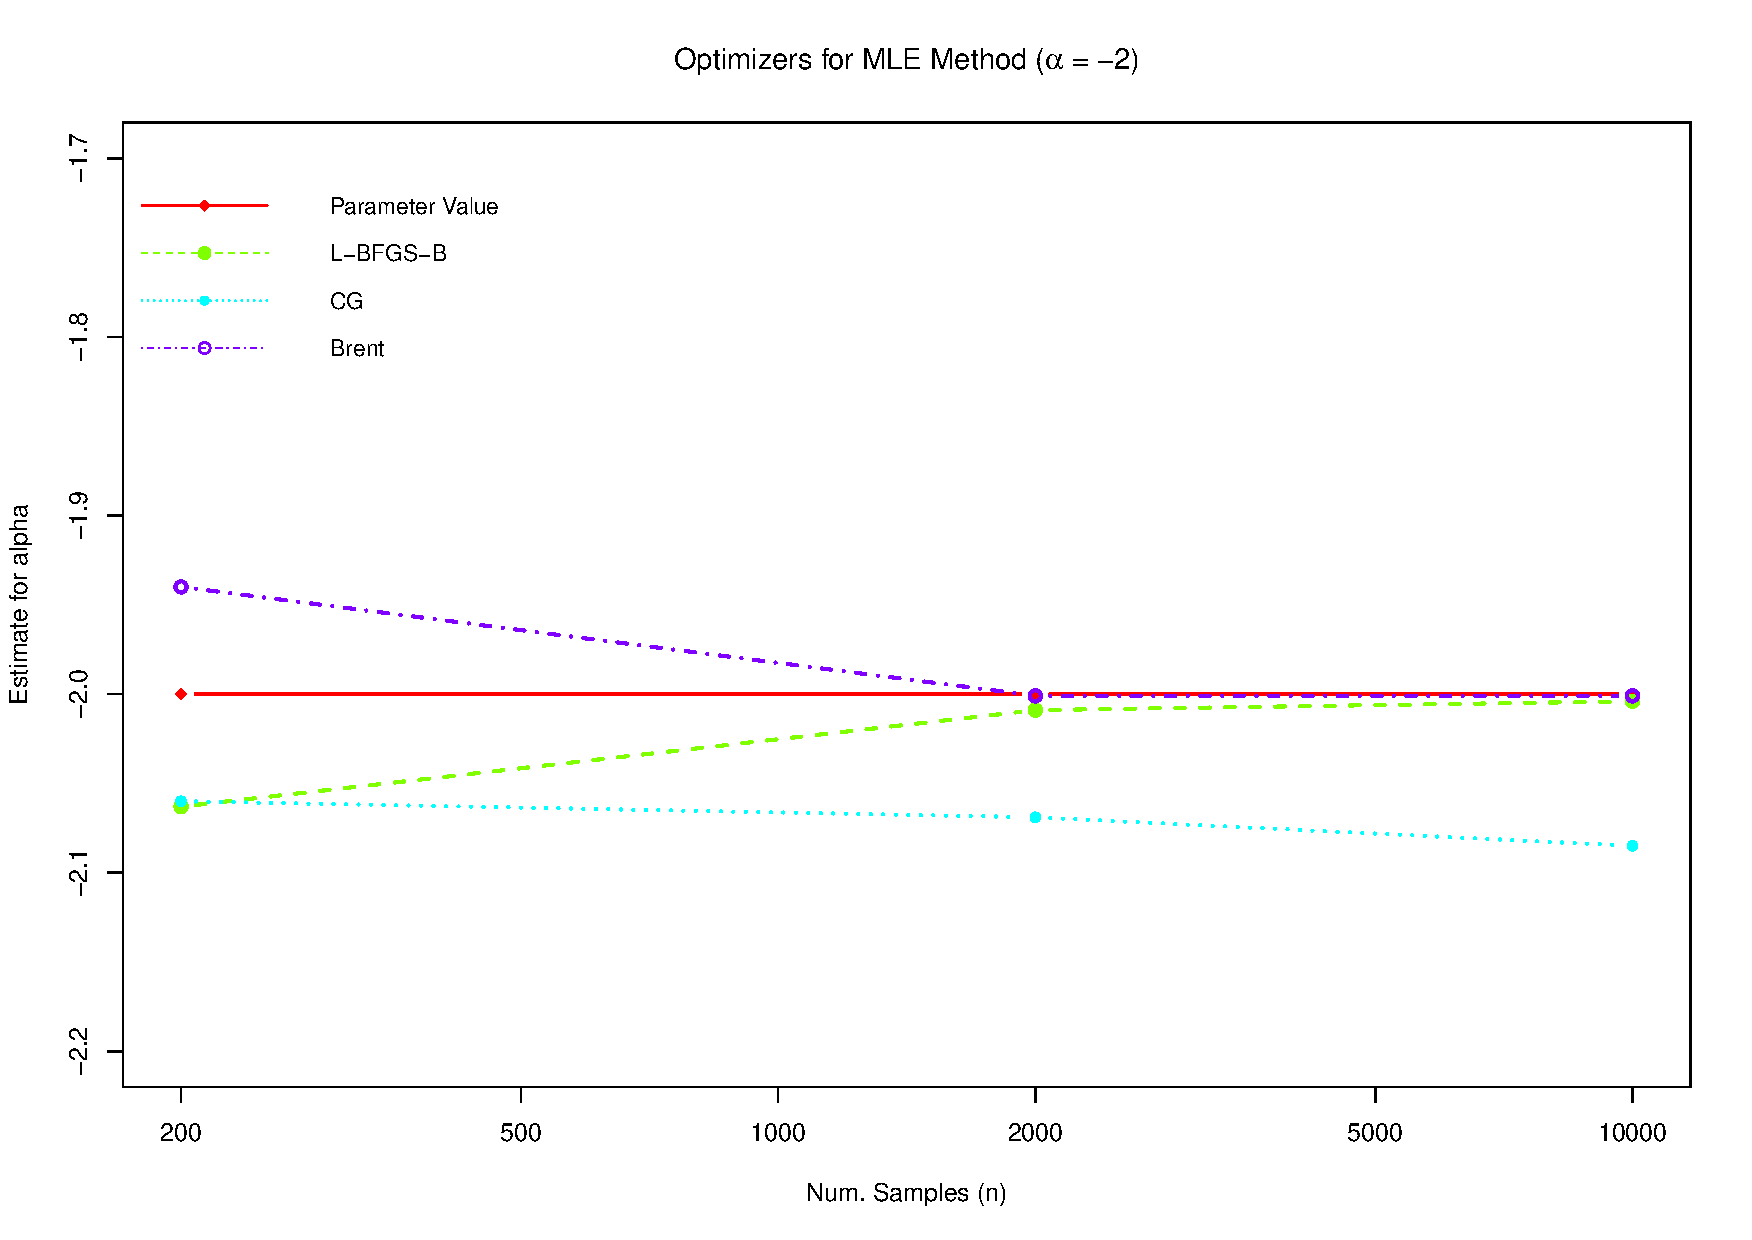
\includegraphics[scale=0.5]{plots/OptimsAlpha-2.pdf}
     \caption{Otimizadores analisados na estimação por MV para $\alpha = -2$}
     \label{graf_2}
\end{figure}
\begin{figure}[H]
     \centering
     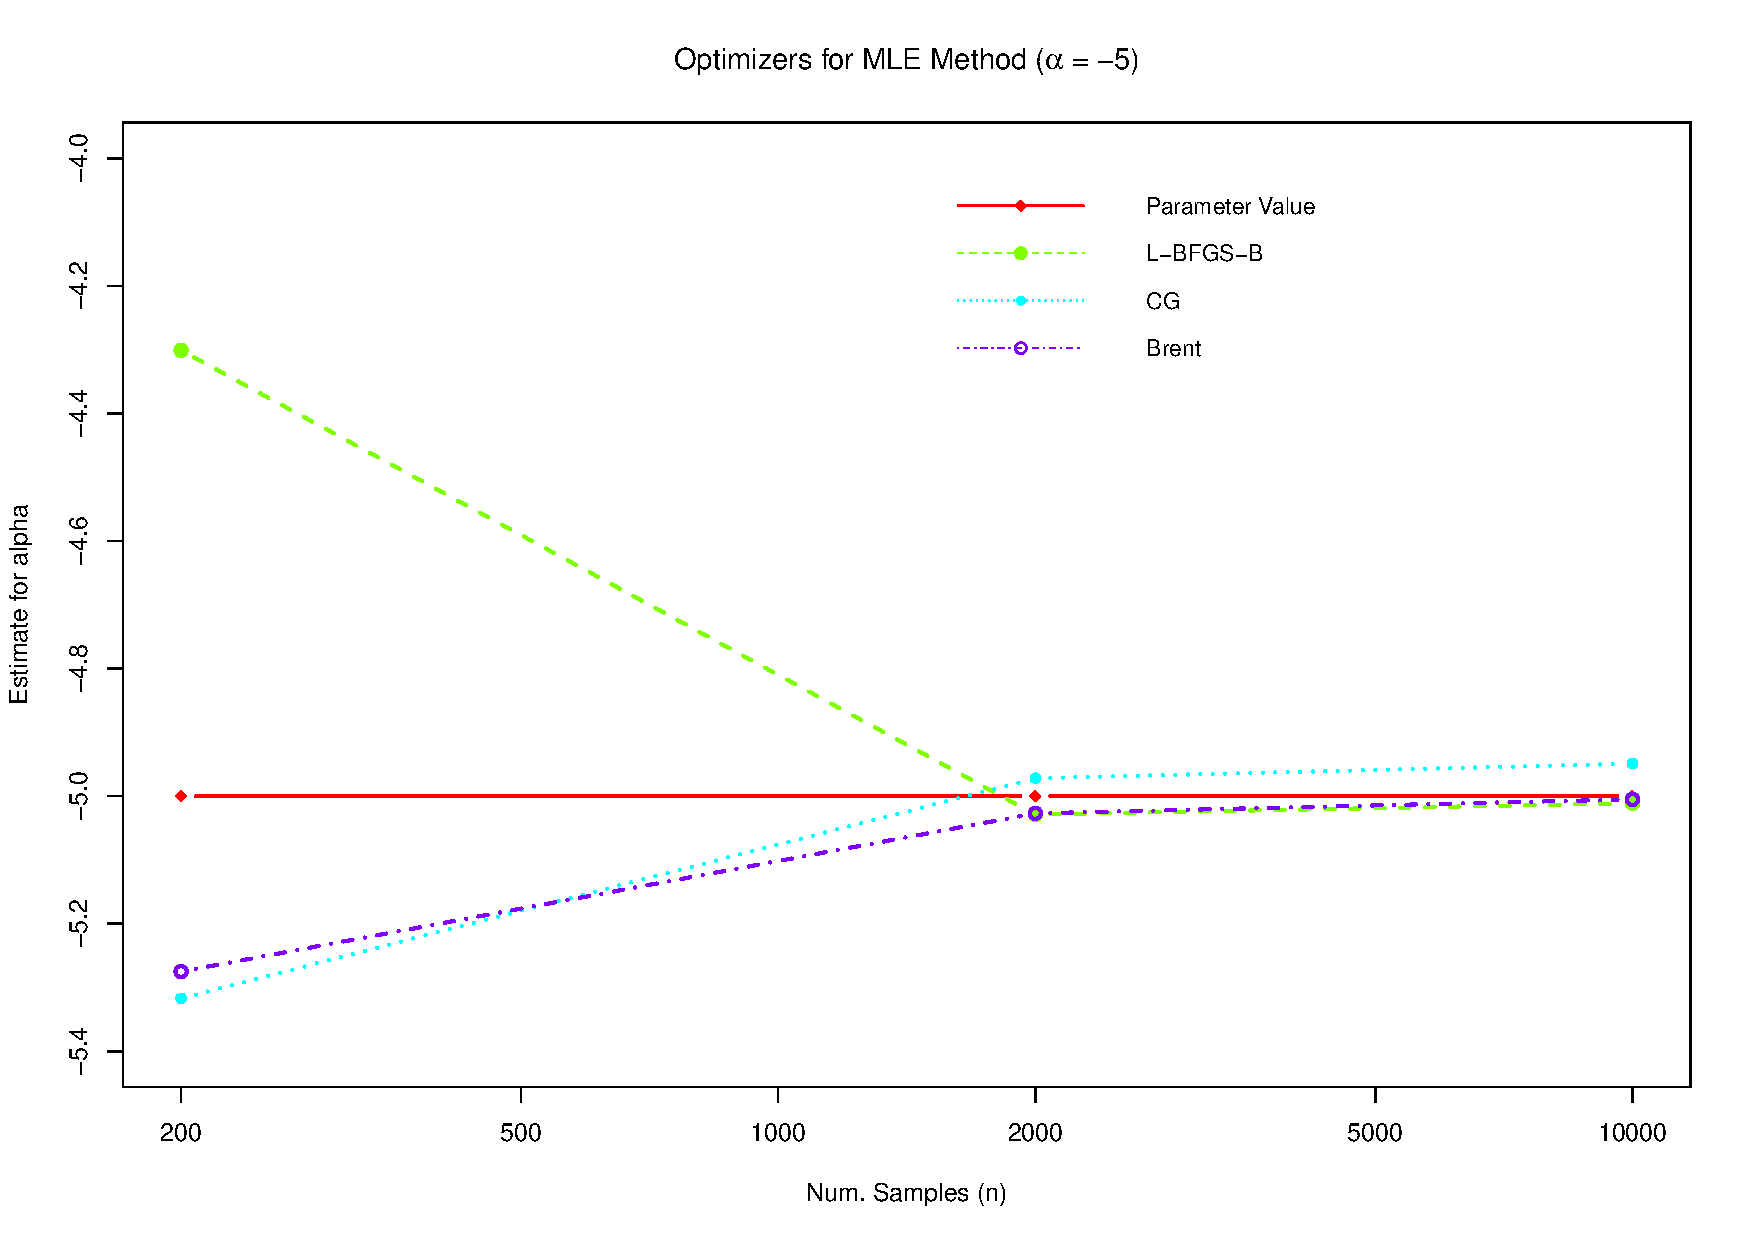
\includegraphics[scale=0.5]{plots/OptimsAlpha-5.pdf}
     \caption{Otimizadores analisados na estimação por MV para $\alpha = -5$}
     \label{graf_3}
\end{figure}
\begin{figure}[H]
     \centering
     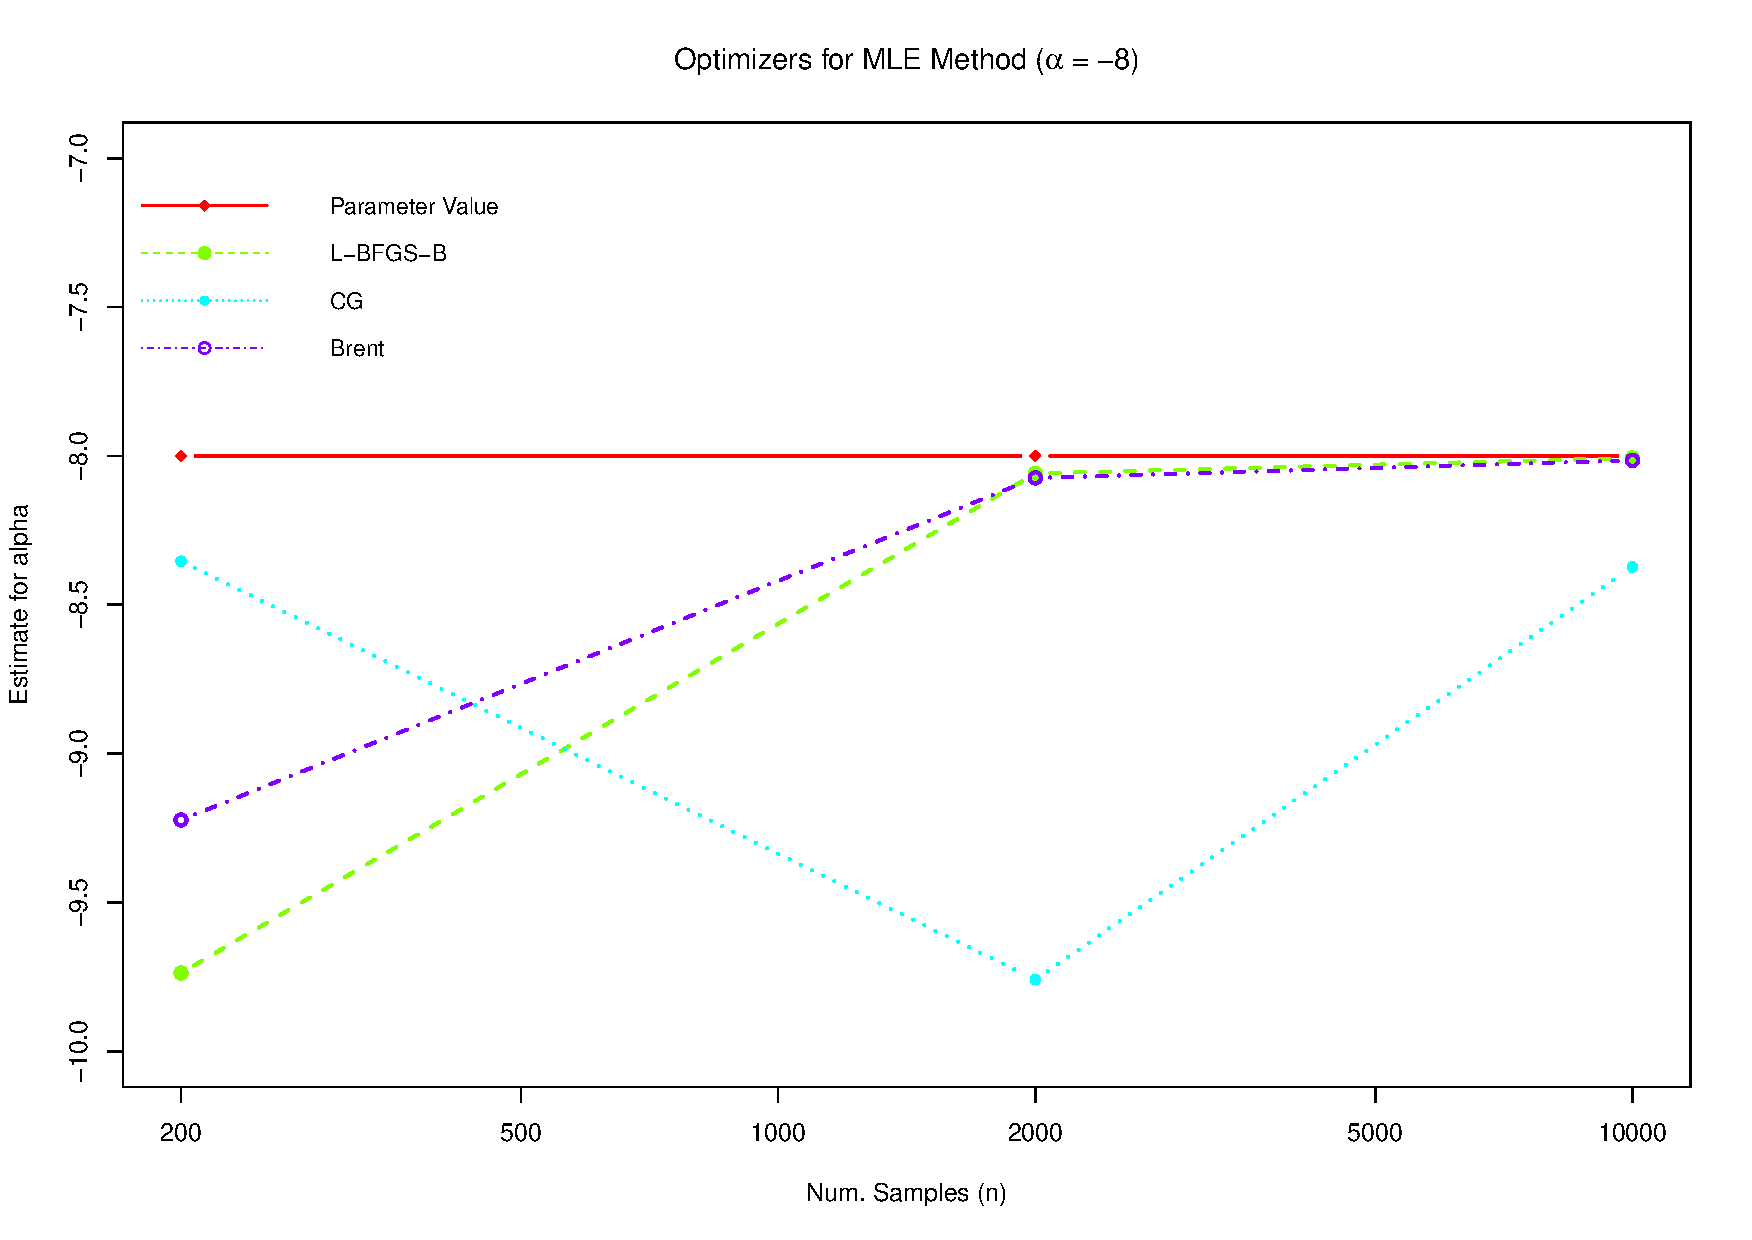
\includegraphics[scale=0.5]{plots/OptimsAlpha-8.pdf}
     \caption{Otimizadores analisados na estimação por MV para $\alpha = -8$}
     \label{graf_4}
\end{figure}

\begin{comment}
Agora temos uma tabela equivalente só que válida para o parâmetro $\gamma$ que foi estimado nos otimizadores \emph{L-BFGS-B} e \emph{CG}.
\begin{table}[H]
\centering
\caption{Estimadores para o parâmetro $\gamma$ ($ \overline{\widehat{\gamma}}$) }
\vspace{0.2cm}
\begin{tabular}{r|r|lr}
\hline
Configuração & L-BFGS-B & CG \\ 
\hline                               
$(200, -2, 7, 3)$ & 7.290 & 7.283  \\
$(200, -5, 7, 3)$ & 7.477 & 7.506  \\
$(200, -8, 7, 3)$ & 8.641 & 7.330  \\
$(2000, -2, 7, 3)$ & 7.050 & 7.266  \\
$(2000, -5, 7, 3)$ & 7.050 & 6.952  \\
$(2000, -8, 7, 3)$ & 7.057 & 8.712  \\
$(10000, -2, 7, 3)$ & 7.019 & 7.324  \\
$(10000, -5, 7, 3)$ & 7.013 & 6.918  \\
$(10000, -8, 7, 3)$ & 7.005 & 7.336  \\
\end{tabular}
\end{table}
\end{comment}

Diante dos gráficos que mostram os resultados obtidos no processo de estimação da $G_I^0$ por Máxima Verossimilhança, podemos observar que todos os otimizadores são bem sensíveis quanto ao tamanho de amostras utilizadas, se mostrando melhores quando o número de amostras é maior, isto é, convergem melhor quando atuam com tamanhos de amostras maiores. Dentre os três otimizadores utilizados os que forneceram melhores estimativas com menores erros foram os otimizadores de \emph{L-BFGS-B} e de \emph{Brent}. No quesito tempo de execução, o \emph{L-BFGS-B} obteve vantagem em relação ao otimizador de \emph{CG}, visto que apresentou menor tempo de execução para executar a simulação Monte Carlo com 1000 replicações. Este fato ocorreu justamente, por conta de sua estratégia de memória limitada, restrigindo o espaço de busca por meio dos limites de fronteira.

O otimizador de \emph{Brent}, embora seja aplicado somente a problemas de otimização unidimensionais com somente um parâmetro sendo passado, também mostrou resultados bem satisfatórios em um tempo muito pequeno. Contudo, por conta da unidimensionalidade, o seu uso é restrito e deve ser utilizado assumindo algumas simplificações o que certamente é uma real desvantagem frente aos demais.

Como conclusão da análise feita, temos que o otimizador mais robusto e mais completo que forneceu os melhores resultados, no menor tempo de execução e sendo possível de ser utilizado com $n$-dimensões foi o \emph{L-BFGS-B}. Para os casos em que podemos tratar os problemas de forma unidimensional, visando encontrar somente um parâmetro desconhecido, podemos aplicar o otimizador de \emph{Brent} que é próprio para tais situações e oferece resultados bem satisfatórios.

\subsection{Implementação do estimador de Momentos}

Como já discutido, estimadores de Momentos são bastante utilizados nos processos de estimação de parâmetros para diversas distribuições. Nesse contexto, vale frisar que os estimadores de momentos fracionarios foram amplamente utilizados com sucesso no trabalho de \citet{Clutter1997}. Com isso, utilizando-se $r = 1/2$ na equação \eqref{eq:moments} basta resolver a equação dada em \eqref{fractional_moments} para obter o valor de $\widehat{\alpha}$. Dessa forma, tendo em mãos este valor, podemos utilizar a simplificação adotada em que obtemos o parâmetro $\gamma$ da $G_I^0$ fazendo o valor esperado ($E(Z)$) valer 1 e, assim, obtemos que o estimador $\widehat{\gamma}$ pode ser calculado como sendo $\widehat{\gamma} = -\widehat{\alpha} - 1$ como já explicado anteriormente.

O estimador de momentos foi implementado com o auxílio do pacote do \texttt{R} chamado \texttt{rootSolve}. Este pacote foi criado para resolver os exemplos de análise de estabilidade e estado estacionário no livro de \citet{Soetaert2009}. Neste pacote, temos o método chamado \textit{uniroot} em que passamos a equação dada em \eqref{fractional_moments} e, dessa forma, obteve-se de maneira simples, rápida e precisa o estimador $\widehat{\alpha}$.

Vale ressaltar que, de modo similar ao procedimento feito com os estimadores de Máxima Verossimilhança descritos anteriormente, foi realizado um experimento de Monte Carlo em que gerou-se um total de 1000 replicações onde as amostras foram geradas para cada ponto do espaço de parâmetros considerado na tabela \ref{tab:tabela_parameters}. Dessa forma, foram produzidos os vetores de estimadores, $\{\widehat{\alpha}_{1}, \widehat{\alpha}_{2}, \dots, \widehat{\alpha}_{1000}\}$. A partir desses vetores, foram então calculados, para cada caso, a média das estimativas, $\overline{\widehat{\alpha}} = (1000)^{-1} \sum_{i=1}^{1000} \widehat{\alpha_{i}}$, e o erro quadrático médio.


Abaixo está a tabela que contém os resultados dos estimadores de momentos encontrados com o procedimento realizado.
\begin{table}[H]
\centering
\caption{Estimadores de Momentos} 
\begin{tabular}{@{\extracolsep{4pt}}c|c|c|c|c}
\toprule   
\multicolumn{1}{c}{\textbf{Amostras}} & \multicolumn{1}{c}{\textbf{Escala}} & \multicolumn{1}{c}{\textbf{Looks}} & \multicolumn{1}{c}{\textbf{Textura}} & \multicolumn{1}{c}{\textbf{Est. de Momentos}} \\
 \cmidrule{1-1} 
 \cmidrule{2-2} 
 \cmidrule{3-3} 
 \cmidrule{4-4} 
 \cmidrule{5-5} 
\multicolumn{1}{c}{$n$} & \multicolumn{1}{c}{$\gamma$} & \multicolumn{1}{c}{$L$} & \multicolumn{1}{c}{$\alpha$} & \multicolumn{1}{c}{$\widehat{\alpha}_{Mom12}$} \\ 
\midrule
200  & 7 & 3 & -2 & -2.209  \\ 
   & ~ & ~ & -5 & -5.254  \\ 
   & ~ & ~ & -8 & -7.211  \\ \hline
2000  & 7 & 3 & -2 & -2.012   \\ 
   & ~ & ~ & -5 & -5.046    \\
   & ~ & ~ & -8 & -8.172   \\ \hline
10000  & 7 & 3 & -2 & -2.001  \\ 
   & ~ & ~ & -5 & -5.069   \\
   & ~ & ~ & -8 & -8.208    \\
\bottomrule
\end{tabular}
\end{table}


\subsection{Implementação do estimador de Log-Cumulantes}

Os estimadores baseados no método de Log-Cumulantes (MLC) foram também encontrados de modo similar ao procedimento realizado para encontrar os estimadores de momentos. Mais uma vez, contou-se com o auxílio do pacote \texttt{rootSolve}, mais precisamente do método \emph{uniroot}, para calcular a raiz da equação \eqref{eq:alphaEst_logCum} descrita anteriormente. De forma análoga, o experimento de Monte Carlo foi desenvolvido para o cálculo dos estimadores. A seguir encontram-se os estimadores de Log-Cumulantes encontrados a partir do procedimento realizado.
\begin{table}[H]
\centering
\caption{Estimadores de Log-Cumulantes} 
\begin{tabular}{@{\extracolsep{4pt}}c|c|c|c|c}
\toprule   
\multicolumn{1}{c}{\textbf{Amostras}} & \multicolumn{1}{c}{\textbf{Escala}} & \multicolumn{1}{c}{\textbf{Looks}} & \multicolumn{1}{c}{\textbf{Textura}} & \multicolumn{1}{c}{\textbf{Est. Log-Cumulantes}} \\
 \cmidrule{1-1} 
 \cmidrule{2-2} 
 \cmidrule{3-3} 
 \cmidrule{4-4} 
 \cmidrule{5-5} 
\multicolumn{1}{c}{$n$} & \multicolumn{1}{c}{$\gamma$} & \multicolumn{1}{c}{$L$} & \multicolumn{1}{c}{$\alpha$} & \multicolumn{1}{c}{$\widehat{\alpha}_{LCum}$} \\ 
\midrule
200  & 7 & 3 & -2 & -2.027  \\ 
   & ~ & ~ & -5 & -4.972  \\ 
   & ~ & ~ & -8 & -7.908  \\ \hline
2000  & 7 & 3 & -2 & -2.004   \\ 
   & ~ & ~ & -5 & -5.094   \\
   & ~ & ~ & -8 & -8.225   \\ \hline
10000  & 7 & 3 & -2 & -2.000  \\ 
   & ~ & ~ & -5 & -5.008   \\
   & ~ & ~ & -8 & -8.064    \\
\bottomrule
\end{tabular}
\end{table}

\subsection{Implementação do estimador de Distâncias Estocásticas}

Como já discutido anteriormente, para implementação dos estimadores obtidos pela Minimização de Distâncias Estocásticas foram necessárias duas etapas: 1) integração numérica necessária para calcular a distância Triangular entre a distribuição empírica e a densidade da $G_I^0$ e 2) otimização do sistema com relação ao parâmetro $\alpha$ de modo a encontrar o valor do parâmetro que minimiza a distância.

Nesse contexto, foi utilizado o pacote da plataforma \texttt{R} chamado \texttt{cubature} e, em especial, a função \texttt{adaptIntegrate} deste pacote para resolver a integral referente ao cálculo da distância Triangular. O algoritmo utilizado é uma integração multidimensional adaptativa sobre hipercubos. Abaixo, encontram-se os estimadores obtidos conforme este procedimento e também após ser feito o experimento de Monte Carlo.
\begin{table}[H]
\centering
\caption{Estimadores de Log-Cumulantes} 
\begin{tabular}{@{\extracolsep{4pt}}c|c|c|c|c}
\toprule   
\multicolumn{1}{c}{\textbf{Amostras}} & \multicolumn{1}{c}{\textbf{Escala}} & \multicolumn{1}{c}{\textbf{Looks}} & \multicolumn{1}{c}{\textbf{Textura}} & \multicolumn{1}{c}{\textbf{Est. Distâncias Estocásticas}} \\
 \cmidrule{1-1} 
 \cmidrule{2-2} 
 \cmidrule{3-3} 
 \cmidrule{4-4} 
 \cmidrule{5-5} 
\multicolumn{1}{c}{$n$} & \multicolumn{1}{c}{$\gamma$} & \multicolumn{1}{c}{$L$} & \multicolumn{1}{c}{$\alpha$} & \multicolumn{1}{c}{$\widehat{\alpha}_{DT}$} \\ 
\midrule
200  & 7 & 3 & -2 & -2.037  \\ 
   & ~ & ~ & -5 & -4.372  \\ 
   & ~ & ~ & -8 & -6.865  \\ \hline
2000  & 7 & 3 & -2 & -1.191   \\ 
   & ~ & ~ & -5 & -4.094   \\
   & ~ & ~ & -8 & -6.534   \\ \hline
10000  & 7 & 3 & -2 & -1.194  \\ 
   & ~ & ~ & -5 & -3.076   \\
   & ~ & ~ & -8 & -6.538    \\
\bottomrule
\end{tabular}
\end{table}

\subsection{Comparação dos estimadores implementados}

A seguir estão os gráficos que mostram uma comparação das estimativas providas pelas técnicas de estimação implementadas neste trabalho: Máxima Verossimilhança, Momentos, Log-Cumulantes e Distâncias Estocásticas.
\begin{figure}[H]
     \centering
     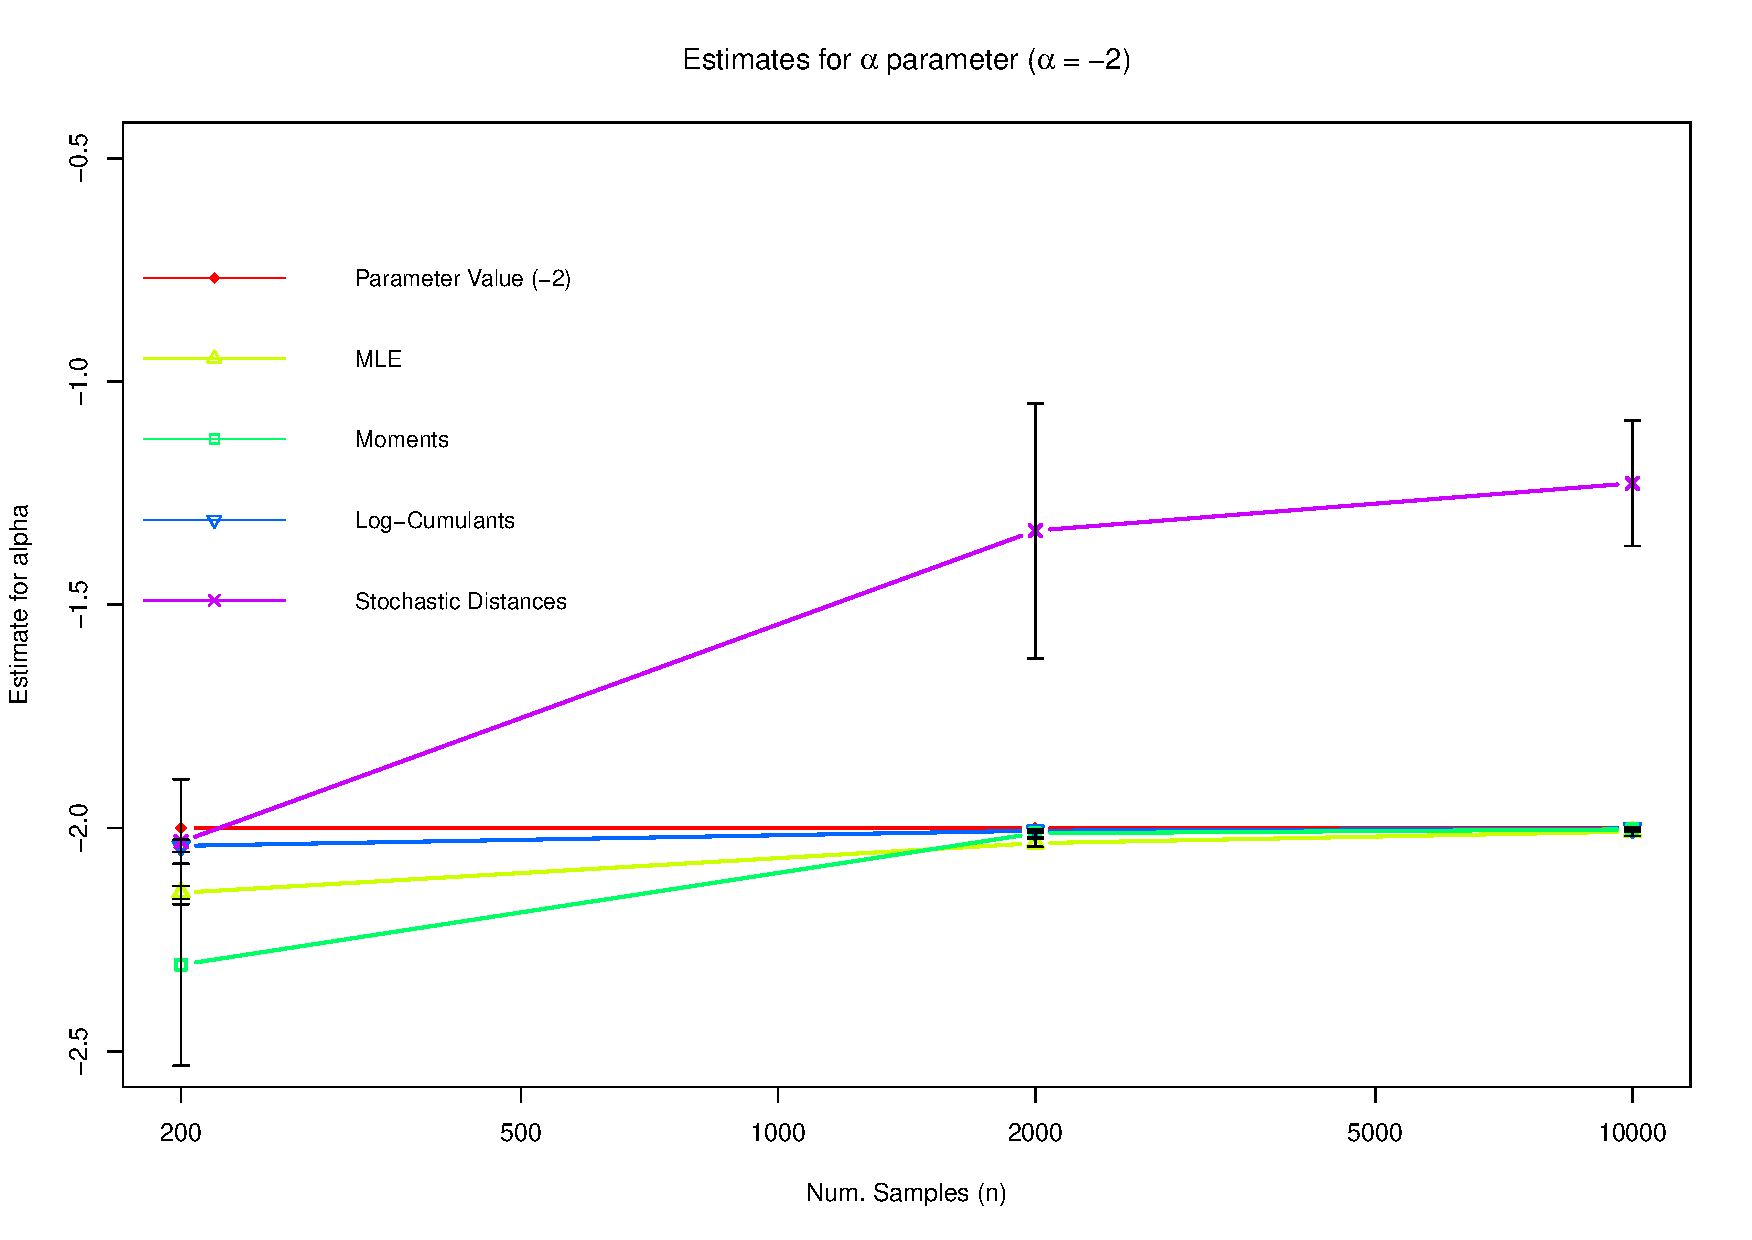
\includegraphics[scale=0.5]{plots/ComparisonAlpha-2.pdf}
     \caption{Estimativas obtidas para o parâmetro $\alpha = -2$}
     \label{graf_5}
\end{figure}
\begin{figure}[H]
     \centering
     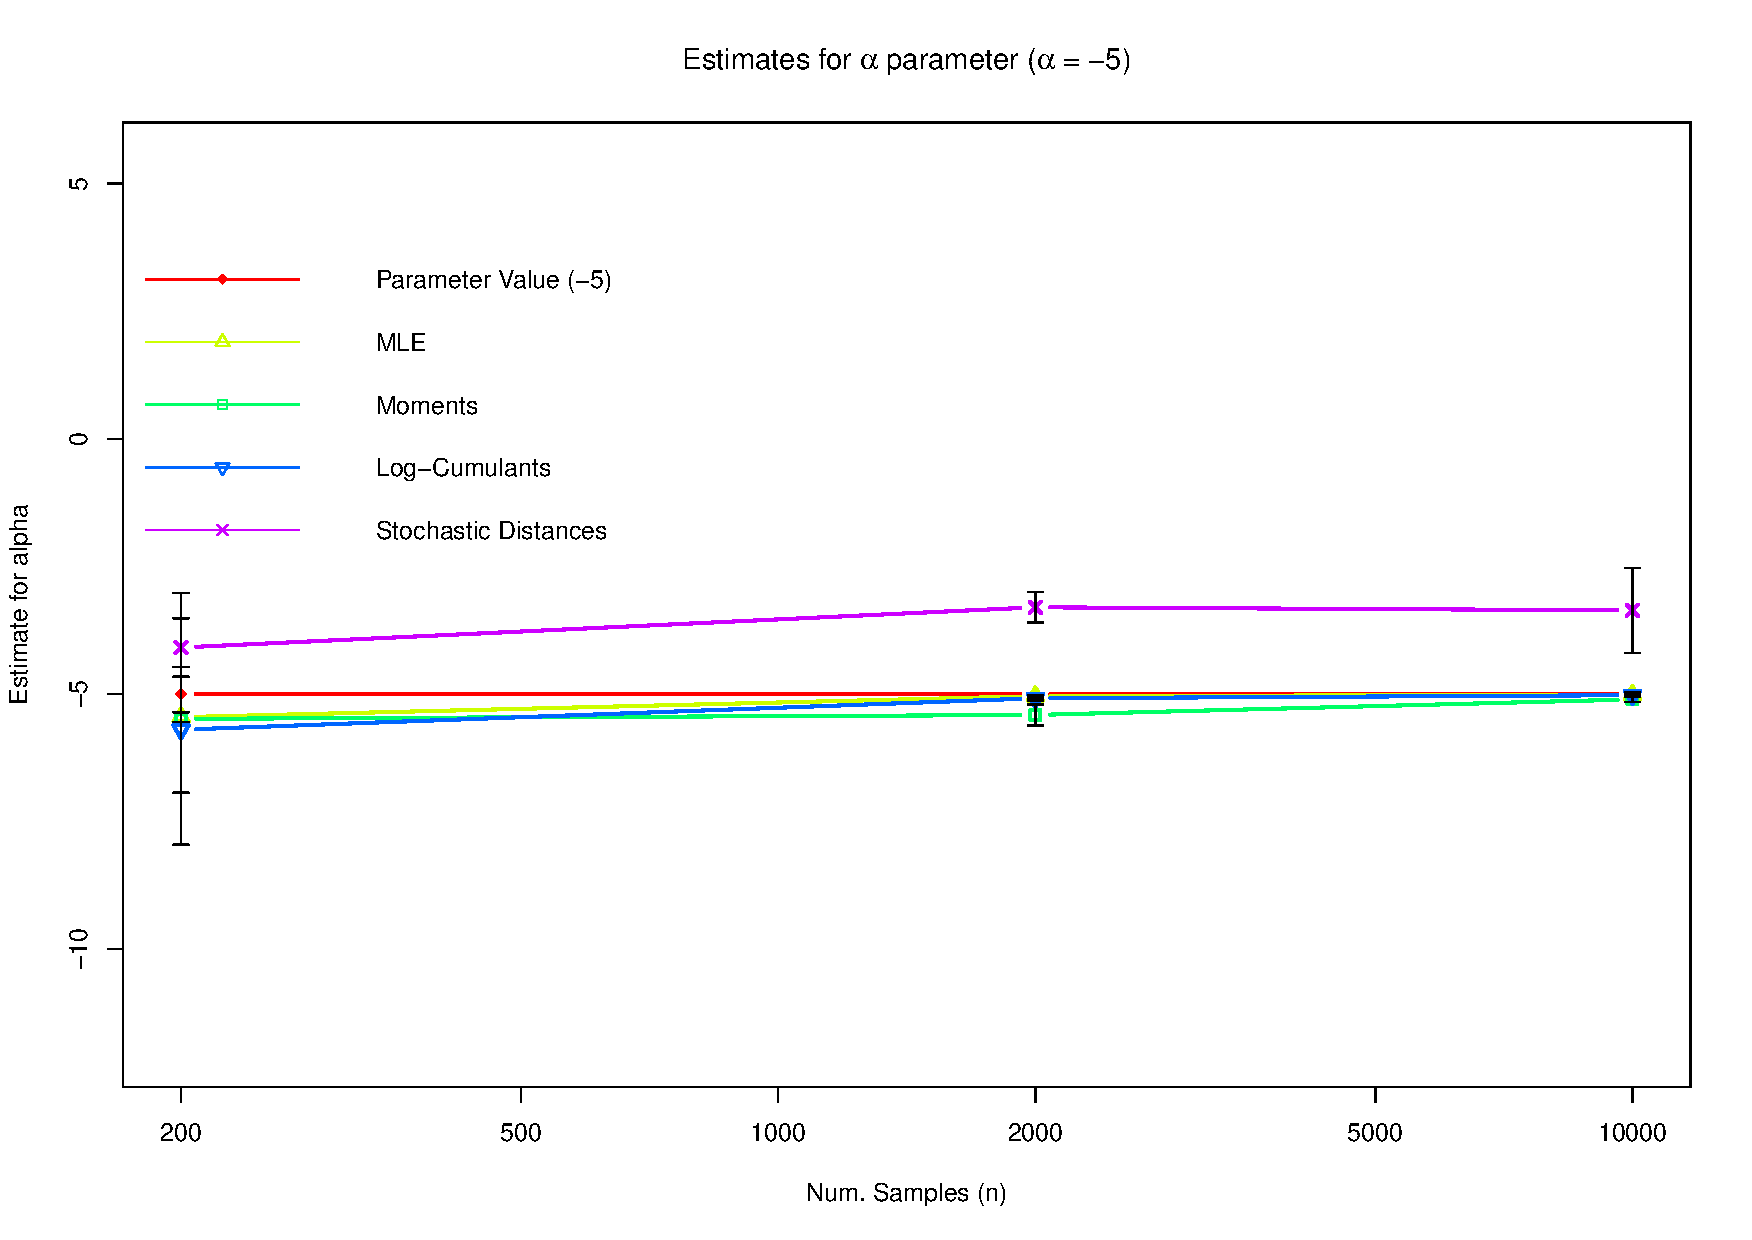
\includegraphics[scale=0.5]{plots/ComparisonAlpha-5.pdf}
     \caption{Estimativas obtidas para o parâmetro $\alpha = -5$}
     \label{graf_6}
\end{figure}
\begin{figure}[H]
     \centering
     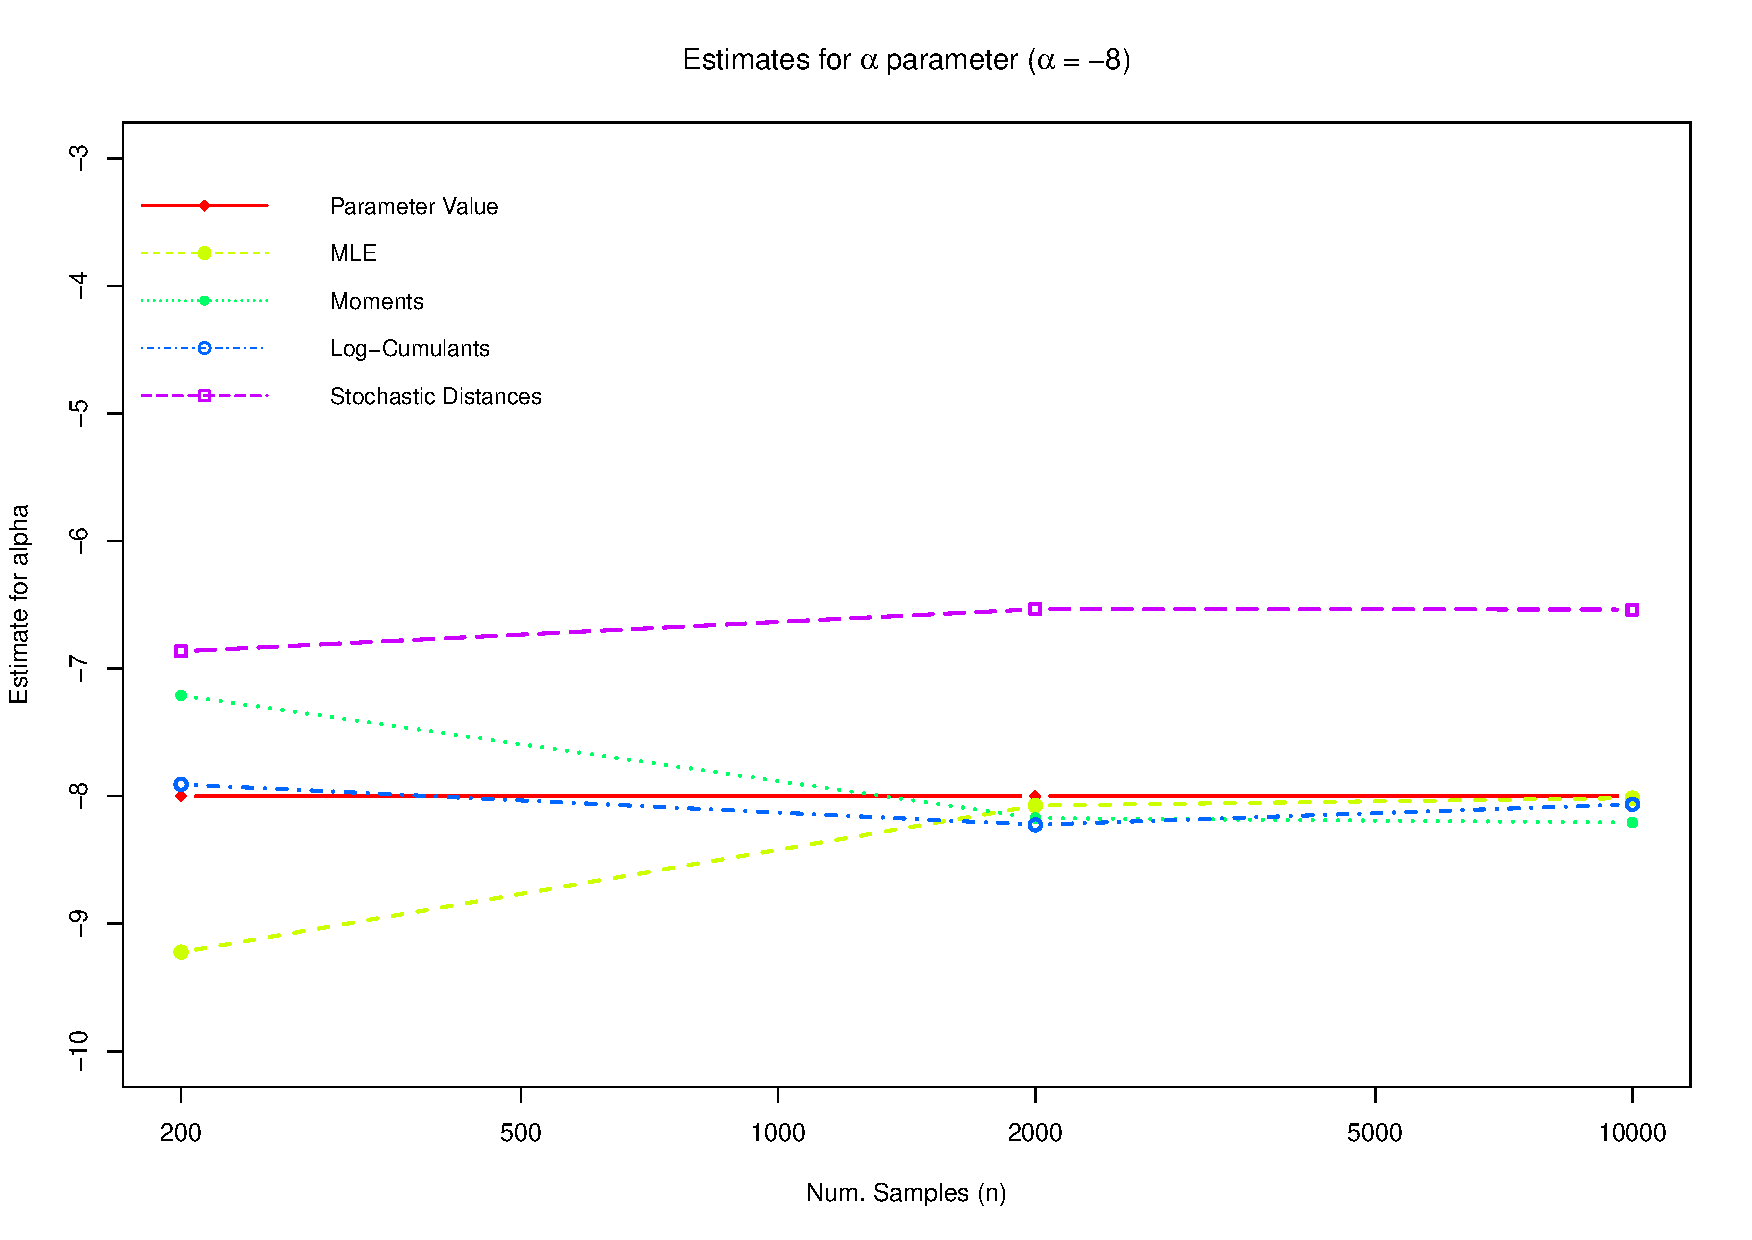
\includegraphics[scale=0.5]{plots/ComparisonAlpha-8.pdf}
     \caption{Estimativas obtidas para o parâmetro $\alpha = -8$}
     \label{graf_7}
\end{figure}


\subsection{Fluxograma de execução da rotina de estimação}
 TO DO

\section{Conclusões}
 TO DO

\section{Trabalhos Futuros}

Diante das técnicas de estimação já implementadas com suas respectivas estimativas já exibidas em tabelas e gráficos, os trabalhos futuros consistem agora em pensar no funcionamento da rotina de estimação que encapsula essas técnicas e escolhe a mais adequada para cada situação.

Os esforços agora serão direcionados para gerar o fluxograma de execução dessa rotina de estimação, em que por meio deste, podemos ter compreensão clara de como o sistema de estimação se comporta diante de cada situação que lhe aparece.




\newpage
\bibliographystyle{agsm}
%\bibliographystyle{unsrt}
\bibliography{../../../Bibliography/references}
%\bibliography{references}


\end{document}